\documentclass[12pt, oneside, a4paper, titlepage]{report}
\usepackage{url}
\usepackage{hyperref}
\hypersetup{%
    hidelinks,
    pdfinfo = {%
        Author = {Paul Mabileau},
        Title = {Rapport de Mission en Entreprise},
        Subject = {Stage de fin d'études},
        Keywords = {%
            rapport,
            stage,
            ingénieur,
            intégration,
            sécurité,
            OCD,
            Orange Cyberdéfense,
        },
    },
}

\usepackage{nameref}
\usepackage{fancyvrb}
\usepackage[toc, acronym]{glossaries}
\usepackage[export]{adjustbox}
\usepackage{booktabs}
\usepackage{longtable}
\usepackage{tabularx}
\usepackage{pbox}
\usepackage[main = french]{babel}
\usepackage{moresize}
\usepackage{xcolor}
\usepackage[utf8x]{inputenc}
\usepackage{csquotes}
\usepackage{graphicx}
\usepackage[section]{placeins}
\usepackage{calc}

\usepackage{geometry}
\geometry{%
    paper = a4paper,  % Paper size, change to letterpaper for US letter size.
    top = 3cm,  % Top margin.
    bottom = 3cm,  % Bottom margin.
    left = 3.5cm,  % Left margin.
    right = 3.5cm,  % Right margin.
    headheight = 0.75cm,  % Header height.
    footskip = 1cm,  % Space from the bottom margin to the baseline of the footer.
    headsep = 0.5cm,  % Space from the top margin to the baseline of the header.
    %showframe,  % Uncomment to show how the type block is set on the page.
}

\usepackage[sorting = none]{biblatex}
\addbibresource{refs.bib}
\setacronymstyle{long-short-desc}
\loadglsentries{glossary.tex}
\makeglossaries{}

\newcommand{\nomPrenom}{{%
    \fontsize{14}{14}\selectfont Paul Mabileau
}}
\newcommand{\nomEntreprise}{{%
    \fontsize{16}{16}\selectfont ORANGE CYBERDÉFENSE
}}

\newcommand{\nomAdresseEntreprise}{{%
    \fontsize{12}{12}\selectfont Orange Cyberdéfense, 2 rue Christophe Colomb,
    91300 Massy.
}}

\newcommand{\titreMission}{{%
    \fontsize{14}{14}\selectfont Intégration sécurité: déploiement d'une
    architecture SD-WAN pour trois sites de production.
}}

\newcommand{\nomDirecteurStage}{{%
    \fontsize{12}{12}\selectfont Valentin Goron
}}

\newcommand{\nomConseillerStage}{{%
    \fontsize{12}{12}\selectfont Olivier Paul
}}

\newcommand{\anneeUniversitaire}{{%
    \fontsize{15}{15}\selectfont 2020/2021
}}

\newcommand{\dateDebut}{{%
    \fontsize{12}{12}\selectfont 22/02/2021
}}

\newcommand{\dateFin}{{%
    \fontsize{12}{12}\selectfont 20/08/2021
}}

\newcommand{\vap}{{%
    \fontsize{11}{11}\selectfont SSR
}}




\begin{document}

\begin{titlepage}
    \newpage
\thispagestyle{empty}


\begingroup
    \begin{tabular}{ll}
        % LOGO DE TELECOM SUDPARIS
        \begin{minipage}[c]{0.0\textwidth}
            \begin{flushleft}
                
\includegraphics[width=3cm]{img/logo/tsp.png}
            \end{flushleft}
        \end{minipage}
        &
        % ANNEE UNIVERSITAIRE
        \hspace{-3em}
        \begin{minipage}[c]{1.0\textwidth}
            \begin{flushright}
                \textbf{ANNÉE \anneeUniversitaire}
            \end{flushright}
        \end{minipage}
        \hspace{\stretch{1}}
    \end{tabular}
    \vskip 3.0em
\endgroup

\begingroup
    \begin{center}
        \Large{\textbf{RAPPORT de <<MISSION en ENTREPRISE>>}}
        \vskip 1.5em

        présenté par:
        \vskip 1.5em
        \textbf{\nomPrenom}

        \vskip 2.5em
        Mission effectuée du \dateDebut{} au \dateFin{} chez
        \vskip 2.0em
        \textbf{\nomEntreprise}
        \vskip 2em

        Sujet de la mission:
    \end{center}

     % CADRE POUR LE TITRE DE LA MISSION
    \parbox[b]{1.0\textwidth-1cm}{%
        \hrule height 1.5pt
        \vrule width 1.5pt
        \hspace{1.80cm}
        \parbox[b]{\textwidth-5cm}{%
            \center\large{\textbf{\titreMission}}\endcenter{}
        }
        \hspace{1.80cm}
        \vrule width 1.5pt
        \hrule height 1.5pt
    }
    \vskip 3.5em
\endgroup

\begingroup
    Directeur de stage: \textbf{\nomDirecteurStage}
    \vskip 1.0em
    Conseiller de Stage: \textbf{\nomConseillerStage{}}
\endgroup

\vskip 4.5em

\begingroup
    \hrule height 1.0pt
    \vskip 0.5em
    \noindent Travail effectué pour la société: \nomAdresseEntreprise{}
\endgroup


\newpage

\end{titlepage}

\setcounter{page}{2}
\tableofcontents

\newpage
\thispagestyle{empty}


\begingroup
    \begin{tabular}{ll}
    % LOGO DE TELECOM SUDPARIS
        \begin{minipage}[c]{0.0\textwidth}
            \begin{flushleft}
                
\includegraphics[width=4cm]{img/tsp.png}
            \end{flushleft}
        \end{minipage}
        &
        % ANNEE UNIVERSITAIRE
        \hspace{-3em}
        \begin{minipage}[c]{1.0\textwidth}
            \begin{flushright}
                \Large{\textbf{Stage de 3\up{ème} année}}\\
                \Large{\textbf{\anneeUniversitaire}}
            \end{flushright}
        \end{minipage}
        \hspace{\stretch{1}}
    \end{tabular}
    \vskip 1.0em
\endgroup

\begingroup
    \noindent \textbf{Nom de l'étudiant}: \nomPrenom{}
    \vskip 0.5em
    \noindent \textbf{VAP}: \vap{}
    \vskip 0.5em
    \noindent \textbf{Entreprise}: \nomEntreprise{}
    \vskip 0.5em
    \noindent \textbf{Dates}: du \dateDebut{} au \dateFin{}
    \vskip 0.5em
    \noindent \textbf{Sujet}: \titreMission{}
    \vskip 3em

    % FR
    \noindent
    \fbox{%
        \parbox{\textwidth}{%
            \vskip 0.8em
            \hspace{0.5cm}
            \vspace{0.4em}
            \large{\textbf{RÉSUMÉ:}}
            \vskip 0.4em
            \vskip 0.8em
        }
    }

    % EN
    \noindent
    \fbox{%
        \centering
        \parbox{\textwidth}{%
            \vskip 0.8em
            \vspace{0.4em}
            \hspace{0.5cm}
            \large{\textbf{ABSTRACT:}}
            \vskip 0.4em
            \vskip 0.8em
        }
    }
    \endgroup


\newpage



\chapter{Remerciements}%
\label{cha:ackn}

Je tiens tout d'abord à remercier mon directeur de stage, Valentin Goron, pour
son suivi régulier du stage et des activités que j'y menais, pour souvent
m'orienter vers une personne prête à m'aider à résoudre un quelconque problème.
Je remercie à ce titre Guerric Lemoigne pour son accueil efficace et son
attention à toutes les petites opérations et questions qui viennent avec un
début de stage, Andrès Marino pour les dépannages en salle serveur, Arnaud
Fauvel pour la rédaction du DEX, Deroi Tieffi pour avoir été un bon taxi,
Geoffrey Giganti pour le coup de pouce pour démarrer en Stormshield, et j'en
oublie d'autres.

Je remercie également les chefs de projet avec qui j'ai eu l'occasion de
collaborer, ne serait-ce qu'un peu: Arnaud Creuser et surtout Laurent Saunier
pour avoir brillamment géré un projet en mouvement constant, bourré de
changements de dernière minute et fréquemment bloqué ou retardé par des imprévus
dépassant nos responsabilités.

Merci aussi à Gauthier pour les longues journées de nos débuts de stage passées
en salle de test à documenter, nettoyer, réorganiser et étiqueter tout ce qui
bouge --- ou en l'occurrence plutôt pas trop.

Enfin, je tiens tout particulièrement à remercier Sylvain Bardy pour un travail
en binôme qu'il rend toujours efficace mais surtout agréable du fait de son
soutien constant et de sa bonne humeur inconditionnelle. Même lorsque contraint
à devoir jongler entre plusieurs projets dont d'autres bien plus prenants, il
était toujours prêt à répondre à mes nombreuses questions et interrogations,
voire à se libérer d'une minute à l'autre pour résoudre divers problèmes
ensemble sans pour autant avoir à le demander. Je pense sincèrement que la
réussite du projet en question et de mon stage peut lui être attribuée en grande
partie. Merci beaucoup.


\chapter{Introduction}%
\label{cha:intro}

\section{Stage}%
\label{sec:intro::stage}

Aujourd'hui, la sécurité est souvent citée comme un enjeu majeur pour les
entreprises ainsi que pour l'ensemble de ses parties prenantes. Elle n'est plus
confinée uniquement au rôle de l'informaticien. Le domaine devient de plus en
plus important à cause de la transition progressive vers des systèmes
informatiques~\cite{reliance}, de l'Internet et de protocoles réseau sans fil
tel que Bluetooth ou Wi-Fi, et de la constante augmentation du nombre
d'appareils <<intelligents>> tels que téléphones et télévisions modernes et les
nombreux types différents d'appareils constituant <<l'Internet des objets>>. Du
fait de sa complexité grandissante, à la fois en termes politiques et
technologiques, la cybersécurité est aussi un des défis proéminents du monde
contemporain~\cite{global-cyber}. Ces raisons amènent alors de nombreuses
entreprises à investir un temps et un budget significatifs à l'établissement
d'une sécurité opérationnelle estimée adaptée aux contraintes liées à leur cœur
de métier. C'est dans ce cadre que s'inscrit l'activité d'Orange Cyberdéfense et
en particulier mon stage.

Mon stage avait pour domaine principal l'\gls{integ} d'outils de sécurité pour
le compte de clients d'Orange Cyberdéfense. Comme ceux-ci sont variés, les
projets associés abordent des sujets plus ou moins spécifiques, des enjeux et
contraintes différents, une criticité de la sécurité adaptée, des durées et
budgets variés, \ldots{} L'idée est donc de les accompagner dans une démarche
d'identification de sujets et problèmes de sécurité les concernant directement,
d'amélioration de leurs infrastructures, logiciels et configurations, et de
conception d'architectures adaptées à l'implémentation de ces changements dans
le cadre d'un projet dédié.

L'\gls{integ} de système est une activité d'ingénierie qui relève du processus
de mise en relation de différents systèmes, souvent disparates, dans le but
qu'ils deviennent composants d'un nouveau système plus global. En informatique,
il peut s'agir de connexions physiques entre machines ou logiques entre
logiciels. En sécurité, cela ajoute certaines contraintes, notamment de ne pas
s'arrêter uniquement au bon fonctionnement du système global mais d'inclure
aussi le non-fonctionnement souhaité de ce qui n'appartient pas au système.


\section{Présentation de l'entreprise}%
\label{sec:intro::entreprise}

\begin{figure}[h!]
    \centering
    
\includegraphics[width = 0.8\linewidth]{img/logo/ocd.png}
    \caption{Logo de la marque \acrlong{ocd}}%
    \label{fig:logo/ocd}
\end{figure}

\Gls{ocd} SAS est une filiale d'\gls{obs}, elle-même filiale et marque
commerciale du groupe Orange. \gls{ocd} est spécialisée dans la prestation de
services en cybersécurité: elle accompagne les entreprises dans la sécurisation
de leurs activités et de leurs données. L'entreprise a son siège dans le
quartier de La Défense, en région parisienne et compte plus de 2500
collaborateurs dont plus de 250 chercheurs et analystes à travers le monde,
répartis dans 160 pays~\cite{ocd}.

\acrlong{ocd} a été fondée en 2014 et dirigée jusqu'en avril 2021 par Michel Van
Den Berghe. La marque est créée en 2016, regroupant les activités en
cybersécurité d'Orange Consulting et d'Atheos, cabinet de conseil racheté en
2014~\cite{rachat-atheos}.  La filiale a ensuite évoluée avec le rachat de Lexsi
en 2016 puis SecureData et SecureLink en 2019 pour une valeur de 515 millions
d'euros~\cite{rachat-securelink}. La direction est reprise en avril 2021 par
Hugues Foulon.

Financièrement et humainement, l'entreprise a connu une forte croissance depuis
sa création. Entre 2016 et 2020, \gls{ocd} a eu une croissance de chiffre
d'affaires de 21,3\% en moyenne, pour atteindre 300 millions d'euros en 2020 et
768 millions d'euros en 2020 aussi en prenant également en compte toutes les
acquisitions de la filiale~\cite{ocd}. Le résultat net quant à lui a quelque peu
oscillé au fur et à mesure des années, mais était par exemple de 2,984 millions
d'euros en 2016, 883 milliers d'euros en 2018 et 1,826 millions d'euros en 2020.
L'effectif salarial est lui aussi en augmentation assez régulière depuis 2015
avec en moyenne 30,0\% de croissance jusqu'à fin 2020, pour atteindre plus de
1100 employés début 2021~\cite{finances-ocd}. L'ensemble du détail des finances
de l'entreprise est mis à disposition en annexe~\ref{sec:annexes::finances-ocd}.

\acrlong{ocd} propose une notable variété de services informatiques en sécurité.
Ils contiennent en particulier au niveau purement technique: du conseil, de
l'audit organisationnel et de sécurité par tests d'intrusion, de la détection de
menaces de manière transparente aux clients et des réponses automatisées, de la
conception d'architectures nouvelles ou en vue d'une migration avec de
l'\gls{integ}, et enfin du support et du \gls{soc} pour atteindre un \gls{mcs}.
Il y a aussi des services plus orientés sur l'axe humain de la sécurité: des
formations visant à sensibiliser les employés d'une entreprise cliente, mais
aussi de l'assistance à la gestion de crise~\cite{ocd}.  Puisque je n'ai fait
partie que de l'équipe d'\gls{integ}, je ne serais en mesure de préciser la
structure interne et le fonctionnement précis des autres équipes. Leur
intervention dans le déroulé d'un projet complet sera cependant abordé en de
plus amples détails dans la partie~\ref{cha:mission} --- \nameref{cha:mission}.

En particulier, l'offre de filtrage délocalisé et réponse automatisée à incident
est réalisée grâce à des infrastructures que l'entreprise a conçues et maintient
elle-même. \acrlong{ocd} héberge au sein de 26 centres de détection dans 13 pays
du monde de quoi analyser en moyenne 50 milliards d'évènements par jour, ce qui
permet notamment de révéler et rapidement clôturer en moyenne plus de 200 sites
Web détectés malveillants par jour.


\section{Acteurs du marché}%
\label{sec:intro::acteurs}

La sécurité informatique est un enjeu majeur pour toute entreprise et surtout
constant dans le temps. En effet, la migration vers une informatique généralisée
rend souvent la surface d'attaque de plus en plus importante. Les attaques
informatiques surviennent en permanence et sont surtout de types très variés.

Rien que dans les ménages français par exemple, les personnes faisant face à des
problèmes de sécurité rencontrent huit catégories d'attaques différentes et
déclarent dans 42,5\% des cas avoir été sujet à du hameçonnage par réception
d'un message invitant à se connecter à un site Web frauduleux et dans 21,4\% des
cas par redirection vers un site frauduleux invitant à fournir des informations
personnelles lors d'une navigation Web~\cite{attack-types}.

Cela concerne tout aussi bien les entreprises du secteur privés: 16\% des
sociétés de 10 personnes ou plus implantées en France déclarent avoir vécu un
incident de sécurité informatique en 2018. Les sociétés de 250 personnes ou plus
sont deux fois plus touchées~\cite{companies-security}. Le simple coût lié à la
gestion de la crise déclenchée par une attaque et aux réparations qui
s'ensuivent est conséquent: il est aux États-Unis en moyenne de 27,4 millions de
dollars et en France de 9,72 millions de dollars USD~\cite{attack-costs}. Cela
les amène alors à investir un budget et un temps considérable pour se protéger
en conséquence: en 2019, 87\% des sociétés de 10 personnes ou plus réalisent des
activités en lien avec la sécurité de leur système d'information. Par ailleurs,
67\% des sociétés ont recours à des prestataires pour réaliser des activités de
sécurité informatique, parfois en sus des employés de l'entreprise, et 20\% les
font réaliser uniquement par leurs propres employés, parmi lesquelles les
grandes entreprises le font à 31\%. Ces activités comprennent notamment de
l'édition de communications internes: 26\% des sociétés ont une documentation
sur les mesures, pratiques ou procédures en matière de sécurité des systèmes
d'information, autant qu'en 2015. C'est le cas de 71\% des sociétés de 250
personnes ou plus. Quelle que soit leur taille, sept sociétés sur dix ont défini
ou révisé cette documentation au cours de l'année
écoulée~\cite{companies-security}.

Cette masse d'entreprises ayant recours à des prestataires de services externes
pour les aider à réaliser toutes ces activités particulièrement chronophages est
alors très importante. Le marché associé est donc évidemment conséquent: en
2020, il a représenté à l'échelle globale environ 133 milliards de dollars
USD~\cite{security-market}, dont 96,3 en services de
consultation~\cite{security-consulting-market}, ce qui inclut la grande partie
des activités d'\gls{ocd} par exemple. \acrlong{ocd} est en plus de cela sur la
plupart des fronts de la sécurité (voir la section
précédente~\ref{sec:intro::entreprise}), puisqu'elle sert plus de 8000 clients
de tous secteurs d'activité~\cite{ocd}. Son marché direct est alors de très
grande taille et les acteurs y participant en grand nombre. Quant à certains en
particulier, nous citerons par exemple Atos et Wavestone pour la partie conseil
et conception d'architectures, Synacktiv et Quarkslab pour la partie audit de
sécurité et tests d'intrusion, ou encore Login Sécurité en partie pour les
opérations de \gls{soc}.


\chapter{Mission}%
\label{cha:mission}

Ma mission était, d'un point de vue assez global, de participer aux divers
projets et activités de l'équipe d'ingénieurs en \gls{integ} faisant partie du
département <<Solutions de confiance>> d'\acrlong{ocd}. Cette équipe est
elle-même composée de deux sous-équipes: le \gls{build} et le \gls{run}.  Le
\gls{build} est chargé d'une partie de la conception de l'architecture à mettre
en place pour répondre aux besoins d'un client, puis surtout de son
implémentation effective qui nécessite souvent une intervention matérielle et
l'établissement de configurations logicielles cibles, pour enfin réaliser une
migration vers le nouveau système. Le \gls{run} quant à lui est chargé d'assurer
le bon fonctionnement du système implémenté par le \gls{build} de sorte qu'il
soit opérationnel la majeure partie du temps, de surveiller la sécurité du parc
informatique en question et donc réaliser le rôle de \gls{soc}, mais aussi de
faire évoluer les configurations logicielles au fur et à mesure des demandes du
client par voie de tickets. J'ai, pour ma part, rejoint l'équipe \gls{build}
pour la durée entière de ce stage.


\section{Déroulé d'un projet}%
\label{sec:mission::deroule-projet}

Ces deux sous-équipes plus d'autres d'\gls{ocd} travaillent ensemble pour
réaliser de nombreux projets. Le déroulé typique d'un projet est le suivant,
principalement orienté du point de vue du \gls{build}:

\begin{itemize}

    \item Optionnellement, les équipes d'audit et de conseil ont révélé des
        problèmes de sécurité que l'entreprise cliente d'\gls{ocd} ne juge pas
        acceptable face aux risques potentiellement encourus par rapport à la
        criticité des applications, systèmes et informations concernés. La
        partie conseil va intervenir surtout pour la gestion des opérations
        suite à la mise en évidence des faiblesses en question, pour définir des
        objectifs les plus clairs possibles en terme de sécurité et pour établir
        une stratégie d'évolution pour les atteindre en temps souhaité.

    \item Un projet peut tout aussi bien commencer à l'inverse par une prise de
        contact du client auprès d\gls{ocd}, par exemple suite à un appel
        d'offres, avec des objectifs déjà proprement définis et pour aller
        directement vers l'implémentation. Il s'agit dans ce cas en général de
        construction d'infrastructures entièrement nouvelles ou d'une migration
        relativement importante de systèmes pour laquelle le client a été en
        mesure d'en identifier la nécessité. Une partie non-négligeable de la
        conception est alors réalisée par les \gls{presales} en collaboration
        avec le client.  Leur rôle va principalement être de comprendre et
        synthétiser les besoins du client pour aller vers un premier jet d'une
        architecture adaptée. Si la taille du parc informatique concerné est
        particulièrement conséquente, un ou plusieurs architectes de systèmes
        peuvent aussi intervenir.

    \item Une fois la majeure partie de l'architecture conçue, le \gls{build}
        commence alors à participer au projet pour tendre vers une spécification
        précise des changements qui vont être réalisés ou de l'infrastructure
        qui va être effectivement implémentée. Ceci commence en général par une
        \gls{rli}. C'est une réunion de coordination interne à \gls{ocd} en
        début de projet pour réaliser une transition entre les \gls{presales} et
        les équipes de \gls{build} afin de transmettre les informations
        importantes. Elle est en général relativement courte car il s'agit
        principalement de se mettre d'accord sur ce qui va être présenté au
        client et ainsi de préparer la \gls{rle}. Cette dernière est une réunion
        de début de projet pour le \gls{build} suite à la \gls{rli} cette
        fois-ci avec le client présent pour d'abord faire rencontrer les
        différentes personnes des deux côtés, puis commencer à préparer une
        spécification précise de l'implémentation à réaliser et le continuer
        selon la taille du projet dans les jours, semaines ou mois suivants lors
        d'une série d'ateliers techniques.

    \item Le \gls{build} ayant réellement commencé le projet, ils vont chercher
        à rédiger une spécification de l'architecture à implémenter et déployer
        afin d'obtenir un accord de la part du client à son sujet et donc ainsi
        d'avoir à portée de main une forme de guide contenant toutes les
        informations à configurer sur les différents composants du système
        global à mettre en place. Cela permet aussi de proposer un cadre pour
        les changements en cours de route: si le client avait bien approuvé la
        spécification effective et qu'\acrlong{ocd} l'implémente en entier ou
        presque mais que le client exprime finalement un mécontentement qui
        demanderait de revoir une grande partie de l'architecture, \gls{ocd}
        peut alors s'en défendre en rappelant l'approbation en question; le
        client devra, s'il le souhaite effectivement, renégocier les contrats et
        acheter de nouveau du temps de travail. Selon la taille du projet, cette
        spécification peut prendre différentes formes:

    \begin{itemize}

        \item Si le projet est particulièrement conséquent car fait intervenir
            de nombreuses équipes, demande de déployer beaucoup de sites,
            nécessite un grande variété de configurations, types d'équipements
            ou logiciels, \ldots{} il est alors fréquent de séparer cette
            rédaction en deux parties: un \gls{hld} puis un \gls{lld}. Un
            \gls{hld} est un dossier regroupant les spécifications de
            l'architecture à implémenter d'un point de vue assez global en
            partant de l'idée générale de départ proposée par les
            \gls{presales}. Il ne s'agit pas de préciser toutes les valeurs
            effectives des options principales de configurations cibles à mettre
            en place: c'est plus le rôle du \gls{lld} qui en découle. Ce dernier
            est un dossier regroupant les spécifications les plus détaillées
            possibles de l'architecture à implémenter telles que modèles de
            machine à déployer, versions de systèmes d'exploitation à installer,
            interfaces, adresses, routes, options, autorisations, règles,
            objets, \ldots{} à configurer. Il est en général une continuation
            directe du \gls{hld} associé. Cette séparation en deux permet
            notamment d'un peu mieux gérer la communication car se fait à
            propose des bons sujets lors des ateliers techniques, mais aussi la
            répartition du temps de travail des ingénieurs car évite si possible
            de nombreux aller-retours entre la spécification et
            l'implémentation.

        \item Si le projet n'est à l'inverse pas trop gros, il est souvent
            envisagé de passer directement à un \gls{dsd}. C'est un dossier très
            similaire à un \gls{lld}, car comportera le même genre de contenu
            précis, mais est plutôt employé lorsque la taille du projet n'est
            pas trop conséquente et permet donc de rédiger directement les
            spécifications de l'implémentation en un temps moins long puisque la
            plupart des sujets abordés lors d'ateliers techniques avec le client
            ne posent pas de problème particulier et ne sont donc pas bloquants.
            Pour résumer, un \gls{dsd} est une forme de fusion entre un
            \gls{hld} et un \gls{lld}.

    \end{itemize}

    \item Une fois la spécification rédigée, ajustée et approuvée par le client,
        l'équipe d'ingénieurs \gls{build} dédiée au projet commence
        l'implémentation. Cela démarre régulièrement par une étape de
        \gls{staging}: placer les équipements dans un environnement de test qui
        s'approche le plus possible de l'environnement de production effectif.
        L'intérêt est que cela permet de vérifier certaines parties du système,
        comme par exemple l'interaction avec une base de données externe, qui
        sont dans un environnement de test plutôt en local sur le même hôte,
        mais aussi d'être en mesure d'avoir un contrôle plus important de
        l'environnement global, comme par exemple vider la base de données et y
        charger des données de test qui couvrent des cas précis. Cela permet
        aussi, lorsque cela peut s'appliquer, de vérifier le bon fonctionnement
        de machines physiques pour gérer en interne les potentiels dégâts liés à
        leur transport. Avec une première configuration embarquée dans les
        équipements, le déploiement dans l'environnement de production peut donc
        se faire de manière plus rapide sur place car il s'agit principalement
        de visser les machines, de les alimenter, connecter et démarrer, mais
        aussi de manière plus sereine car une bonne partie des cas ont déjà été
        vérifiés. Après cette étape, l'architecture est déployée et configurée
        petit à petit jusqu'à atteindre un état cible ou presque.

    \item Quand l'implémentation arrive à sa fin, le \gls{build} commence à
        rédiger en parallèle un \gls{dtv} par site déployé. Il regroupe un
        ensemble de fiches de tests d'acceptation à effectuer avec succès pour
        considérer le déploiement du site et la migration globale comme des
        succès, et ainsi que le site soit considéré comme livré au client. Ces
        tests peuvent très bien être entièrement automatisés ou bien faire
        intervenir une certaine part d'actions manuelles: c'est en général le
        cas pour les vérifications de bascule lorsque que la redondance physique
        fait partie de l'architecture globale.  Les différents \glspl{dtv} sont
        complétés et validés par le client au fur et à mesure de quelques
        itérations, comme la majeure partie des documents produits.

    \item Après que le \gls{dtv} d'un site est bien validé et que son
        implémentation est terminée par le \gls{build}, une \gls{vabf} est
        planifiée et effectuée avec le client. Il s'agit d'une session lors de
        laquelle tous les tests d'acceptation du \gls{dtv} associé sont exécutés
        et leur résultats respectifs rapportés dans le document. Si un nombre
        particulièrement important de tests échouent, il est tout à fait
        envisageable de réaliser une nouvelle itération d'implémentation et par
        la suite de planifier et exécuter une seconde \gls{vabf} entière. Si
        seulement un nombre relativement faible de tests échouent, que certains
        n'ont simplement pas pu être réalisés puisque des éléments humains ou
        techniques manquaient ou que certains sont considérés non satisfaisants
        --- c'est-à-dire une forme d'échec partiel où dans certaines conditions
        estimées non courantes les systèmes ne fonctionnent pas comme attendu,
        il est alors possible de considérer la \gls{vabf} comme un succès avec
        quelques retenues tout de même. Les problèmes sont réglés dans les jours
        qui suivent par le \gls{build} et vérifiés en dehors d'une seconde
        \gls{vabf}.

    \item Si les résultats de tous les tests sont des succès, la \gls{vabf} est
        bien complétée, les ingénieurs \gls{build} sont libérés du projet et le
        site en question entre dans une période dite de \gls{vsr}. Pendant cette
        période d'une durée définie en accord avec le client, celui-ci utilise
        l'environnement de production cible déployé et fonctionnel du point de
        vue des tests déjà effectués, mais cette fois-ci pour vérifier que cela
        reste le cas dans la durée, c'est-à-dire qu'il n'y ait pas de
        comportement erratique ou d'instabilité seulement à certains moments de
        la journée par exemple, ou lorsque les systèmes sont soumis à de fortes
        charges, ou encore de temps en temps de manière totalement stochastique.
        Cette durée est en général de deux semaines pour les projets
        d'\acrlong{ocd}, mais peut être étendue principalement sur demande du
        client pour des projets dont ce genre d'aspects est jugé
        particulièrement critique au bon fonctionnement global du système
        considéré. Lors de la \gls{vsr}, l'équipe de \gls{build} réalise les
        corrections demandées par le client en mode <<meilleur effort>>,
        c'est-à-dire que les ingénieurs en question vont y passer le temps
        qu'ils peuvent, mais n'en feront pas pour autant une priorité puisqu'ils
        ne sont plus affectés au projet concerné et peuvent très bien faire déjà
        partie d'un autre projet. Cependant, si un dysfonctionnement majeur se
        produit et qu'il s'agit d'une erreur de la part de l'équipe, \gls{ocd}
        se doit de refaire une itération de \gls{build}, mais s'il s'agit d'un
        problème qui ne leur est pas attribuable, le client devra alors payer
        pour une nouvelle itération s'il le souhaite.

    \item Optionnellement, un \gls{dex} est rédigé en parallèle et sur demande
        du client. C'est une compilation systématique des procédures et des
        opérations que l'administrateur ou l'opérateur du système effectue. Un
        tel dossier leur sert aussi souvent de référence, autant pour du partage
        d'informations que de base pour leur travail quotidien. Il peut
        également contenir des descriptions pour le traitement de demandes
        spéciales et d'éventualités, mais aussi de petits changements à réaliser
        eux-mêmes. Cela permet notamment de clarifier, documenter l'architecture
        effectivement implémentée \textit{versus} celle initialement prévue dans
        un éventuel \gls{dsd}. Ce genre de document est en général produit
        lorsque le client va être en mesure d'administrer son propre système
        potentiellement sans aucune intervention de la part du \gls{run}, et
        pour ainsi lui fournir l'ensemble des éléments pratiques nécessaires de
        sorte que toutes ses opérations régulières puissent être réalisées.

    \item Quand toutes ces étapes-là sont bien finalisées, le projet est en
        quelque sorte terminé, mais l'interaction entre \gls{ocd} et le client
        continue cependant par une transition vers le \gls{run}. Après une
        passation des informations importantes des équipes du \gls{build} vers
        le \gls{run}, ce dernier prend pleinement possession des interventions à
        réaliser sur le parc informatique précédemment déployé et ainsi assurer
        le rôle de \gls{soc} si cela fait partie du contrat négocié avec le
        client. Quelconque modification souhaitée par le client, si encore une
        fois il n'a pas exprimé et négocié dans le contrat le besoin d'aussi
        pouvoir gérer les systèmes soi-même, nécessitera alors qu'il ouvre un
        ticket auprès du \gls{build} afin que ces derniers appliquent le
        changement souhaité. Un tarif au ticket ou groupe de tickets est
        appliqué.

\end{itemize}

En somme, ce mode de travail est assez similaire à la méthode dite de la
<<cascade>> où les étapes sont enchaînées sans vraiment prendre en compte la
possibilité de retour en arrière et encore moins de cycle, ou en tout cas ne pas
la souhaiter. Même si elle a en théorie certains avantages, puisqu'elle cherche
à formaliser les choses à l'avance afin de simplement suivre le flot <<naturel>>
des évènements, elle implique tout de même certaines absurdités. En effet, si on
cherche à la respecter de la manière la plus stricte possible et que, par
exemple, on se rende compte d'une erreur dans la spécification lors de
l'implémentation voire des tests, que fait-on? on continue la chaîne en
outrepassant le problème? on abandonne le projet? on démissionne? Même si on
relâche un peu la définition, cela n'est en fait pas très adapté à certains
projets, comme nous le verrons plus tard. Évidemment, une solution est de
changer de méthode en appliquant par exemple le <<cycle en V>>, au moins de
manière partielle, mais selon mon expérience chez \gls{ocd}, je n'ai pas
l'impression qu'il s'agisse vraiment de l'approche suivie. Cependant, je pense
aussi qu'il n'est pas non plus idéal d'aller à l'extrême opposé, c'est-à-dire de
considérer que rien n'est prévisible et de s'appuyer sur un cycle fréquent pour
effacer les bosses soulevées par des problèmes de conception qui en réalité
auraient pu être prévus. Un minimum de conception à l'avance est toujours
possible et même plus que souhaitable.


\section{Objectifs}%
\label{sec:mission::objectifs}

\acrlong{ocd} étant principalement un prestataire de service, une bonne partie
des objectifs du stage n'ont pas pu être définis à l'avance et de manière
précise, puisque les activités que j'y ai menées dépendaient fortement des
clients et de leur projets en cours. On peut tout de même mettre en évidence les
points suivants:

\begin{itemize}
    \item Apprendre en auto-formation à utiliser les divers produits faisant
        partie des spécialités \gls{ocd} et pouvant être concernés par un de ses
        projets pour aller vers une maîtrise et ainsi participer aux projets en
        tant qu'ingénieur.
    \item Concevoir et implémenter des architectures sécurisées.
    \item Élaborer des documentations techniques, spécifications générales et
        détaillées.
    \item Réaliser des projets: ingénierie, déploiement, migration / mise en
        production, transferts de connaissances, \ldots{}
    \item Contribuer à des activités purement internes telles qu'améliorer les
        infrastructures des salles de test, y déployer de nouvelles maquettes,
        participer au développement de nouvelles expertises, \ldots{}
\end{itemize}


\section{Premières missions}%
\label{sec:mission::prems}

\subsection{Auto-formation}%
\label{sub:mission::prems::auto-formation}

La toute première partie de mon stage consistait en un apprentissage sur une
durée d'un peu plus de deux semaines en auto-formation. Il s'agissait de monter
en compétences sur les quelques technologies apparaissant fréquemment d'un
projet client à un autre, restant assez génériques et ne nécessitant pas de
connaissances particulièrement avancées par rapport à ce qui peut être attendu
d'un futur diplômé d'une école d'ingénieur. Certaines des technologies listées
ci-après ont été étudiées après la première période, mais cela restait fait en
autonomie.

Premièrement, à la demande explicite de mon directeur de stage, je me suis
penché sur Fortinet et plus spécifiquement leur pare-feu FortiGate.  Fortinet
est une entreprise américaine multinationale basée en Californie et qui propose
divers produits de cybersécurité tels que pares-feux, antivirus, systèmes de
détection et prévention d'intrusions et sécurité des terminaux~\cite{forti}.
Leur produit principal reste cependant leur gamme de pares-feux \gls{fgt} que
j'ai donc étudiée grâce à leur formations en ligne~\cite{fgt}. Je me suis aussi
formé sur leur solution de gestion centralisée \gls{fmg}~\cite{fmg} et leur
système de récolte et analyse centralisée de journaux \gls{faz}~\cite{faz}. J'ai
ensuite abordé les produits Palo Alto Networks~\cite{pan}. Cette autre
multinationale américaine aussi basée en Californie propose des produits
principalement centrés sur leur pares-feux~\cite{pan-pa}, notamment en
\textit{cloud}. Enfin, j'ai dû m'intéresser pour le même projet à Microsoft
Azure, hébergeur public et fournisseur de \textit{cloud}~\cite{azure}.

\subsection{Documentation de la salle de tests}%
\label{sub:mission::prems::doc-salle-tests}

En parallèle, un autre stagiaire et moi avions été chargés d'une série de
petites opérations à réaliser pour la salle de tests. Les bureaux de Massy sont
équipés d'une <<petite>> salle serveur comprenant une douzaine de baies pouvant
contenir chacune une quarantaine d'unités standards. Une unité de \textit{rack},
souvent abrégée \textbf{U} ou \textbf{RU}, est une unité de mesure pour les
tiroirs ou \textit{racks} d'une baie de déploiement pour divers appareils en
général informatiques~\cite{rack-unit}. Une telle baie contient typiquement 42
unités. La salle de tests est principalement utilisée pour déployer des
maquettes pour des projets client afin de servir d'environnement de
pré-production (\gls{staging}).  Elle permet aussi aux différents ingénieurs
\gls{build} et \gls{run} de mettre en place leurs propres essais dans le but par
exemple de se familiariser avec les produits d'un fabriquant donné ou bien
encore d'en soumettre à de grosses charges afin de déterminer si les capacités
théoriques annoncées sont en pratique vérifiées.

Les bureaux de la région parisienne ayant emménagés relativement récemment dans
les locaux de Massy, la salle de tests avait été transportée et installée en un
temps un peu trop court pour tout faire au mieux. Certaines des infrastructures
ont donc été mises en place de manière incomplète ou mal documentée. Notre rôle
en début de stage était alors de réaliser une revue la plus complète possible
des baies du \gls{build} et surtout celles dont certaines parties contenaient
des équipements internes, c'est-à-dire ne faisant pas partie d'une maquette
client. Nous devions vérifier que les choses étaient bien installées comme il le
fallait et retirer ce qui n'avait désormais plus sa place dans la salle.
Ensuite, nous nous sommes occupés d'assurer une meilleure documentation des
baies en étiquetant la majeure partie des équipements présents ainsi que les
divers câbles les reliant. Nous en faisions de même dans les configurations des
équipements en changeant leur nom d'hôte et en ajoutant des descriptions à leurs
interfaces si possible. Enfin, nous avons dû réaliser un inventaire des baies et
de la réserve adjacente afin de résumer tout ce qui existe dans l'environnement
de test et ce qui est disponible à l'installation.


\section{Deuxième mission: projet SNCF}%
\label{sec:mission::deuz}

La deuxième mission qui m'a été confiée aura été de participer à la rédaction
d'un \acrfull{dex} dans le cadre d'un projet en approche de fin pour le compte
de la \gls{sncf}. Le projet, nommé <<\textit{Access}>> consistait en la mise en
place d'une architecture publique \textit{cloud} avec l'objectif de fonctionner
en tant que zone tampon pour les flux provenant de l'Internet public et à
destination des applications \gls{sncf} publiques. Ces applications étaient
souvent des applications Web, mais n'y étaient pas restreintes car tout type
était permis tant qu'il était transporté par \gls{tcp} ou \gls{udp}. Cette zone
de sécurité avait pour but l'analyse avancée du trafic, à travers du \gls{waf}
et de l'\gls{ips}.  Elle devait également permettre l'évasion vers l'Internet du
trafic provenant des \glspl{dmz} publiques et privées. Un aperçu de
l'architecture globale est rendue disponible en
Figure~\ref{fig:sncf-access/arch}.

\begin{figure}[h!]
    \centering
    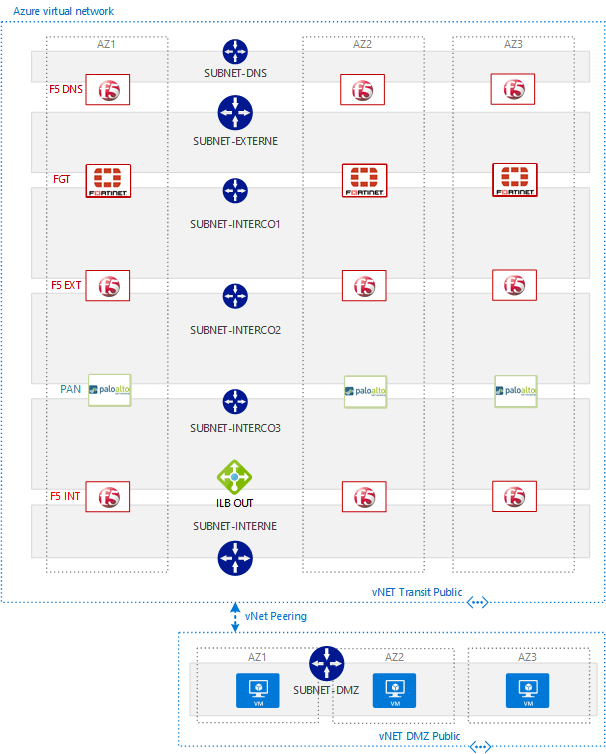
\includegraphics[width = 0.9\linewidth]{img/sncf-access/arch.png}
    \caption{%
        Vue d'ensemble de l'architecture du projet SNCF \textit{Access} sous
        \textit{Azure}%
    }%
    \label{fig:sncf-access/arch}
\end{figure}

Cette architecture suit principalement un modèle en couches pour assurer une
protection à divers niveaux, tels que réseau, applicatif et antivirus. Une
description de ces couches suit:

\begin{itemize}
    \item Un niveau de \acrlong{fgt} est utilisé comme pare-feu externe. Il est
        en charge du filtrage fin niveau 3/4 des flux au sein d'\textit{Access}.
    \item Un niveau de F5 est utilisé comme second bastion. Il est en charge du
        \gls{waf}, avec du déchiffrement \gls{tls} souvent appelé
        <<déchiffrement \gls{ssl}>>.
    \item Un niveau de Palo Alto est utilisé comme troisième bastion. Il est en
        charge de l'analyse \gls{ips}.
    \item Un niveau de F5 est utilisé comme quatrième bastion. Il est en charge
        du re-chiffrement des flux et fonctionne en tant que \gls{rev-proxy}
        pour rediriger le trafic vers les serveurs adéquats.
    \item Un groupe de F5 DNS est utilisé afin d'assurer la résilience entre
        chaque niveau d'équipements.
\end{itemize}

Le \gls{dex} demandé sortait légèrement de la norme habituellement employée pour
la plupart des autres projets. Au lieu de demander un résumé des opérations
d'exploitation, ce qu'ils avaient déjà en partie reçu avant mon arrivée sur le
projet, ils souhaitaient cette fois-ci plus une forme de guide d'implémentation
de nouveaux services. Il s'agit donc moins d'une documentation liée à
l'exploitation des infrastructures déployées, mais plutôt à leur modification en
cas de changement relativement mineur du point de vue du système global. Cela
leur était possible car faisait tout simplement partie des livrables du projet:
la \gls{sncf} souhaitait être en pleine mesure de contrôler ses systèmes.

Nous nous sommes alors chargés de rédiger ce document afin de répondre à la
demande du client. L'axe principal était orienté autour de: comment déployer un
nouveau service au niveau d'\textit{Access}? Nous devions donc détailler le plus
précisément possible l'ensemble des étapes à réaliser à cette fin et ce, pour
chacune des couches définies ci-dessus. Cela impliquait notamment d'inclure
diverses captures d'écran, tableaux résumant certaines informations primordiales
aux étapes concernées, explications et rappels généraux, instructions
spécifiques, \ldots{} Je m'étais personnellement occupé des parties concernant
les opérations sous \acrlong{fgt} pour lesquelles j'ai pu utiliser mes
connaissances fraîchement acquises et celles sous Azure et Palo Alto pour
lesquelles j'ai dû me former tel que mentionné à la
Section~\ref{sub:mission::prems::auto-formation}.  J'ai par ailleurs dû
manipuler directement les ressources de ces quelques technologies déjà déployées
en production afin de produire la majeure partie des sections du document dont
j'étais chargé, même si cela restait assez limité comparé à la mission
principale détaillée en Section~\ref{sec:mission::main}.


\section{Mission principale: projet Hynamics}%
\label{sec:mission::main}

\subsection{Considérations générales}%
\label{sub:mission::main::gen}

Hynamics est une filiale du groupe \gls{edf} fondée en avril 2019~\cite{hy}.
Elle se spécialise dans la production de dihydrogène ($H_2$ et par abus de
langage simplement <<hydrogène>>) renouvelable et à basse émission de dioxyde de
carbone ($CO_2$). Puisque c'est une entreprise assez jeune, peu de choses
visibles concrètement n'avaient été réalisées avant l'été 2021. Ses deux
premières années ont été consacrées à la conception de leurs plates-formes, la
formation de partenariats pour la construction et la production, la mise en
place de contrats à l'avance, etc\ldots{} C'est au début de l'été 2021
qu'Hynamics commence à déployer ses sites de test et de production, en restant
en France pour une première étape. Ces sites ayant besoin d'accès à l'Internet
de manière spécifique et \gls{edf} ayant une culture de la sécurité assez
développée et présente du fait de leurs applications particulièrement critiques,
Hynamics a contacté \acrlong{ocd} afin de sécuriser leurs infrastructures.

Hynamics possède en début de projet trois sites qui en feront partie: le
<<quartier général>> à La Défense (raccourci DEF) qui ne portera pas vraiment de
production ni industrielle ni informatique à proprement parler, un espace sur la
plate-forme de test <<Les Renardières>> (RNRD) d'\gls{edf} près de Fontainebleau
et le premier site de production près d'Auxerre (AUXR). Les objectifs d'Hynamics
pour ces infrastructures étaient de:

\begin{itemize}
    \item Isoler les sites de l'Internet public le plus possible.
    \item Empêcher les sites de communiquer entre eux.
    \item Isoler les uns des autres les équipements des partenaires installés
        sur site le plus possible.
    \item Relier les sites de production au site de La Défense pour permettre
        une gestion centralisée et la remontée des journaux.
    \item Permettre l'accès aux sites en VPN <<\gls{ssl}>> aux collaborateurs
        d'Hynamics et certains de ses partenaires en ayant fait la demande.
    \item Permettre l'accès aux sites en montant des \glspl{tun-ipsec} avec des
        équipements distants de partenaires pour les opérations automatisées.
    \item Obtenir une haute disponibilité acceptable.
\end{itemize}

\begin{figure}[h!]
    \centering
    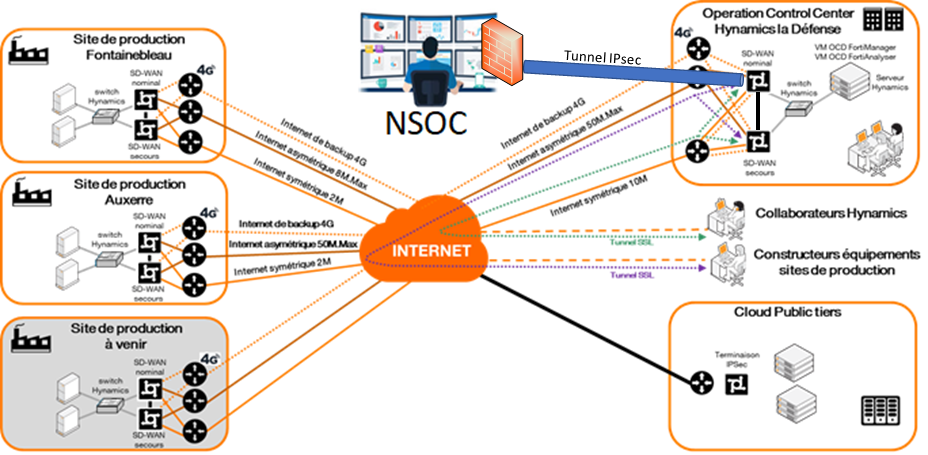
\includegraphics[width = \linewidth]{img/doc-hy/global-arch.png}
    \caption{Architecture globale du projet Hynamics}%
    \label{fig:doc-hy/global-arch}
\end{figure}

L'architecture présentée en Figure~\ref{fig:doc-hy/global-arch} montre le
premier jet conçu par les \gls{presales}. Il montre une vue d'ensemble de ce qui
sera par la suite détaillé et implémenté. Voici quelques détails supplémentaires
à propos de l'architecture qui découlent de la proposition faite par les
\gls{presales}:

\begin{itemize}
    \item Chaque site possède un pare-feu principal qui s'occupe d'agir en tant
        que routeur pour le réseau local et ainsi sa passerelle par défaut pour
        tout accès externe. Il fournit la majeure partie de la sécurité d'un
        site dans ce projet.
    \item Chaque réseau local, sauf celui de La Défense, possède un commutateur
        configurable et capable de gérer les \glspl{vlan}, c'est-à-dire
        manipuler l'extension Ethernet IEEE 802.1q correctement. Cet aspect
        permet de fournir l'isolation souhaitée entre les équipements des
        différents partenaires présents sur sites.
    \item Pour assurer la haute disponibilité (\gls{ha}) demandée, chaque site
        est équipé de trois liens d'accès Internet différents: un premier lien
        filaire \gls{fi} souvent une ADSL, un second \gls{bi} souvent une SDSL
        et un dernier lien cette fois-ci en espace libre par 4G.
    \item De même, le pare-feu de chaque site est en fait une paire du même
        modèle dont les pare-feux sont reliés par une connexion \gls{ha} directe
        permettant la synchronisation automatique des configurations pour rendre
        la paire quasiment identique et la détection automatique de perte de
        l'autre.
    \item Le site de La Défense n'a pas de \glspl{vlan}, mais seulement une
        machine qui héberge deux machines virtuelles: une pour le \acrfull{fmg}
        et l'autre pour le \acrfull{faz}.
    \item Le \acrfull{soc} est relié par un tunnel au site de La Défense afin
        d'être en mesure de surveiller et contrôler tous les autres sites au
        travers des tunnels qui les relient à La Défense.
\end{itemize}

Le modèle de pare-feu retenu par Hynamics avec les \gls{presales} est le
Fortinet \acrlong{fgt} 40F. Il s'agit d'un des modèles faisant partie de la
gamme la moins puissante de Fortinet: les choses ont été faites de ce côté-là le
plus à la baisse possible car cela suffisait en nombre de ports physiques mais
aussi en termes de capacités de traitement puisqu'Hynamics n'avait pas formulé
de besoins de débit particulièrement élevés, la disponibilité importait plus.
Un aperçu du modèle est montré en Figure~\ref{fig:doc-hy/fgt-40f}.

\begin{figure}[h!]
    \centering
    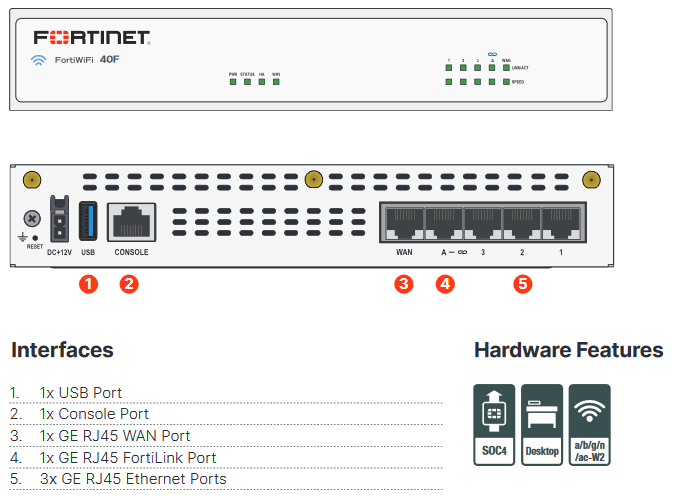
\includegraphics[width = 0.8\linewidth]{img/doc-hy/fgt-40f.png}
    \caption{Aperçu du modèle \acrlong{fgt} 40F}%
    \label{fig:doc-hy/fgt-40f}
\end{figure}

L'architecture physique des sites est présentée en
Figure~\ref{fig:doc-hy/site-phys-arch}. Les deux pares-feux de la paire sont
reliés à tous les routeurs des liens internet disponibles sur le site et au
commutateur central. Ils sont aussi reliés entre eux par un lien \gls{ha}.

\begin{figure}[h!]
    \centering
    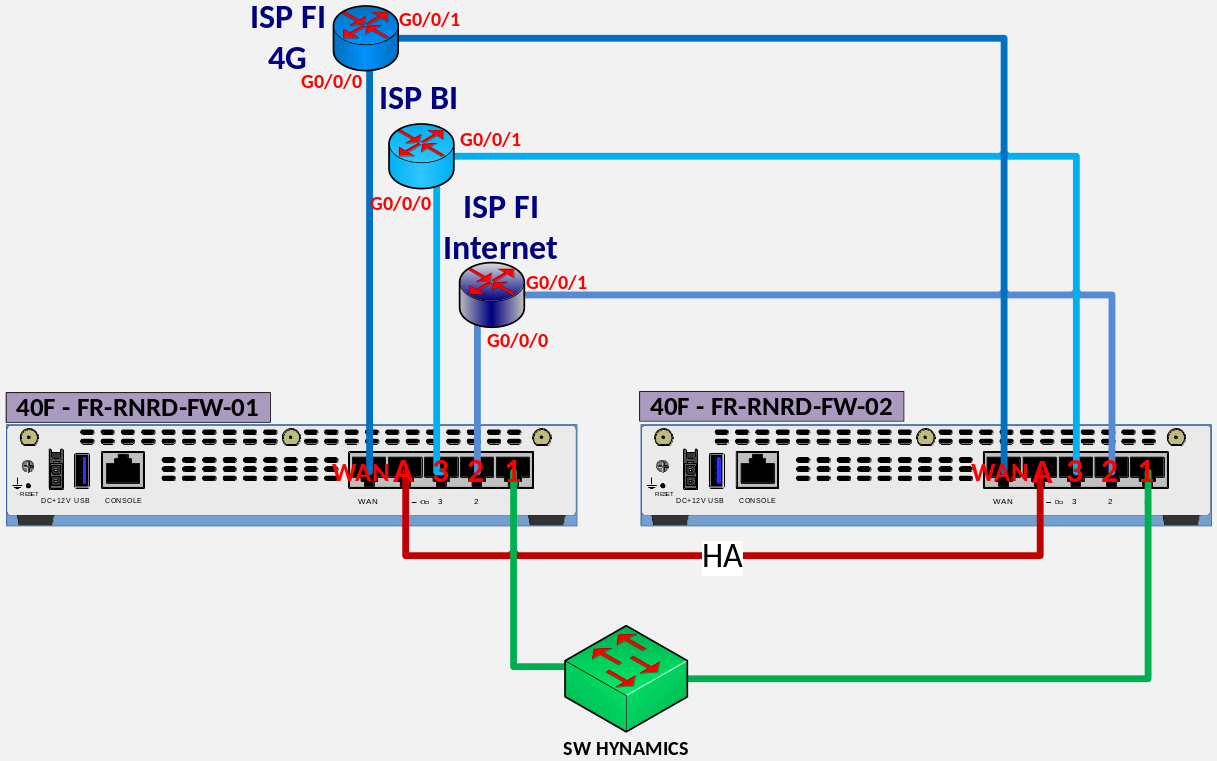
\includegraphics[width = 0.8\linewidth]{img/doc-hy/site-phys-arch.png}
    \caption{Architecture physique d'un site, ici Fontainebleau}%
    \label{fig:doc-hy/site-phys-arch}
\end{figure}

L'architecture logique des sites est présentée en
Figure~\ref{fig:doc-hy/site-logi-arch}. Elle montre comment sont organisés les
différents réseaux et \glspl{vlan} d'un site par rapport aux interfaces
physiques. Chaque partenaire possède son propre \gls{vlan} et son sous-réseau
comme domaine d'adressage pour mettre en place le partitionnement souhaité. Les
\glspl{vlan} sont placés sous l'interface physique \texttt{lan1}.

\begin{figure}[h!]
    \centering
    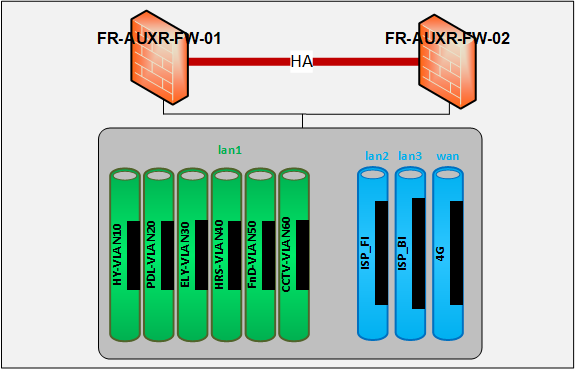
\includegraphics[width = 0.8\linewidth]{img/doc-hy/site-logi-arch.png}
    \caption{%
        Architecture logique d'un site, ici Auxerre avec ses différents réseaux%
    }%
    \label{fig:doc-hy/site-logi-arch}
\end{figure}

\subsection{Démarrage et premières opérations}%
\label{sub:mission::main::start}

Le projet commence pour le \gls{build}, tel qu'expliqué un peu plus tôt à la
Section~\ref{sec:mission::deroule-projet}, par une \acrfull{rli} relativement
courte lors de laquelle les membres internes sont introduits et présentés. Les
\gls{presales} nous transmettent aussi les informations importantes et le
contenu du projet jusqu'à ce jour. La présentation utilisée pour la \gls{rle} du
lendemain est affinée en séance. Celle-ci, la \acrfull{rle}, est effectuée avec
des collaborateurs d'Hynamics présents pour faire les introductions de manière
similaire et clarifier l'état actuel du projet. Les ateliers techniques sont
planifiés pour les jours à venir.

Ces ateliers ont pour but global de concevoir l'architecture de plus en plus
précisément et directement avec le client. Une bonne partie des informations
spécifique au client, c'est-à-dire métier, est cependant obtenue plutôt par
écrit que par oral en réunion car plus efficace.  Cet aspect est abordé plus
amplement dans la Section~\ref{sub:mission::main::collec} suivante. Les ateliers
techniques ont aussi pour objectif d'expliquer certains des protocoles,
technologies, fonctionnalités ou même paradigmes spécifiques à la sécurité afin
que le client soit en mesure de prendre de bonnes décisions éclairées lorsque
nécessaire et de fournir des informations pertinentes lorsque demandées. En
effet, Hynamics est une entreprise petite et récemment fondée: il n'y a pas ou
pas encore de collaborateur ayant reçu de formation particulièrement poussée en
réseau ou en sécurité. Certaines des compétences nécessaires à la compréhension
de quelques aspects du projet n'étaient donc pas présentes chez Hynamics, mais
cela n'était pas spécialement handicapant, cela ajoutait simplement quelques
petits défis supplémentaires. D'autres aspects apparus en cours de projet n'ont
évidemment pas pu être expliqué dès le début, comme nous le verrons un peu plus
tard. Parmi ces choses à expliquer, deux étaient cruciales au projet: le
\gls{vpn-tls} et les \glspl{tun-ipsec}.

Le \gls{vpn-tls} est une forme de \gls{vpn} où un client rejoint virtuellement
un réseau privé en se connectant à un serveur distant visible publiquement et en
y faisant passer ses données au travers. \gls{tls} assure la confidentialité,
l'intégrité et une partie de l'authentification de la communication. Il s'agit
en général de celle du serveur grâce à un certificat. Celle du client est
spécifique à l'implémentation particulière: elle peut être réalisée grâce à une
paire nom d'utilisateur / mot de passe ou un certificat client suivi d'un
échange défi-réponse entre le serveur et le client. Une fois l'utilisateur
authentifié auprès du serveur, ce dernier lui affecte une adresse locale et
récupère une liste de routes auxquelles est inscrit le client et les lui fait
parvenir. Le client crée alors une interface de type tunnel sur son hôte avec
l'adresse reçue et applique aussi les routes reçues de sorte que tout processus
cherchant à réaliser une communication à destination du réseau privé distant
puisse bien la faire puisque le noyau du système gère ce routage. Par exemple,
si un client se connecte au serveur d'adresse publique \texttt{1.2.3.4} afin de
rejoindre le réseau \texttt{172.20.42.0/24}, le serveur lui affectera l'adresse
locale \texttt{172.20.42.252} imaginons. Une fois les informations détaillées
ci-dessus reçues par le client, il crée une interface tunnel d'adresse
\texttt{172.20.42.252/24} et une route où le réseau destination est
\texttt{172.20.42.0/24}, la passerelle \texttt{1.2.3.4} et l'interface émettrice
celle crée juste avant. Cette interface est sous écoute de l'implémentation du
client qui gère toutes les communications effectives avec le serveur. Ainsi
toutes les communications à destination de \texttt{172.20.42.0/24} se font bien
puisque le noyau les redirige vers le client, et le reste n'est pas perturbé
puisque la route ne redirige que ce qui est à destination du réseau en question.
Cette caractéristique de maintien de communications séparées est souvent nommée
en anglais <<\textit{split tunneling}>>.  Évidemment, il est tout à fait
possible de l'empêcher: il suffit de préciser côté serveur que la seule route à
envoyer est \texttt{0.0.0.0/0}, c'est-à-dire le réseau qui englobe toutes les
adresses IPv4 possibles. Ce mode de fonctionnement est souvent utilisé en
entreprise pour être en mesure d'observer tout le trafic de ses employés pour
filtrer le plus de contenu possible et ainsi obtenir une sécurité renforcée,
entraînant parfois du désagrément pour les utilisateurs. OpenVPN est un exemple
d'implémentation libre de ce type de \gls{vpn}. FortiClient est utilisé dans ce
projet puisque spécifique aux produits Fortinet.

Un \gls{tun-ipsec} ou plus précisément dans le cadre de ce rapport <<tunnel
IKE/ESP>>, c'est-à-dire le mode tunnel de la suite \gls{ipsec}, est une autre
forme de \gls{vpn} où deux routeurs établissent une connexion pour mettre en
relation virtuellement deux sous-réseaux privés par-dessus un réseau public. Le
protocole \gls{ike} est utilisé pour construire les clés et \gls{esp} pour
transporter les paquets de manière sécurisée. \gls{ike} est un protocole utilisé
par \gls{ipsec} pour mettre en place une \gls{sa} et qui utilise des certificats
ou clés pré-partagées pour construire un secret commun par Diffie-Hellmann et
ainsi en dériver des clés cryptographiques. Une \gls{sa} est l'établissement
d'attributs de sécurité partagés par deux entités de réseau pour permettre des
communications sécurisées, tels qu'un algorithme cryptographique et son mode de
fonctionnement ou une clé de chiffrement et d'autres paramètres dédiées aux
données à transmettre au travers de la connexion. Cette étape est souvent
appelée <<phase 1>>. \gls{esp} est un protocole de la suite \gls{ipsec} qui, en
mode tunnel, encapsule entièrement les paquets IP à transporter dans de nouveaux
paquets IP\@. Il permet de fournir authenticité en authentifiant la source,
intégrité grâce à des fonctions de hachage cryptographiques et confidentialité
grâce au chiffrement des paquets IP chargés.  Cette étape est souvent nommée
<<phase 2>>. C'est cette encapsulation qui permet de créer le réseau virtuel
sans affectation d'adresse locale ni de traduction d'adresse. En effet,
lorsqu'un hôte émet un message depuis le réseau privé de départ, il le fait avec
comme adresse source la sienne et la destination celle dans le réseau privé
d'arrivée. Il envoie ce paquet au routeur local puisqu'il l'a comme passerelle
configurée automatiquement ou bien manuellement au moins pour atteindre le
réseau de destination, si ce n'est pour tous les réseaux externes. Le routeur
réalise ensuite les opérations d'\gls{esp}: chiffre le paquet et le met comme
charge utile d'un nouveau paquet dont la source est l'adresse publique du
routeur de départ et la destination celle publique du routeur d'arrivée. Ce
paquet est transporté par le réseau partagé, par exemple l'Internet public,
jusqu'au routeur d'arrivée qui réalise les opérations inverses: déchiffre la
charge et l'émet sur le réseau privé local. Celui-ci transporte le paquet
précédemment encapsulé vers la destination qui est alors en mesure de répondre
exactement de la même manière, puisque la connexion et les configurations sont
symétriques.

Un schéma résumant la différence entre \gls{vpn-tls} et \gls{tun-ipsec} d'un
point de vue réseau assez basique et haut niveau est disponible en
Figure~\ref{fig:misc/tls-vs-ipsec}.

\begin{figure}[h!]
    \centering
    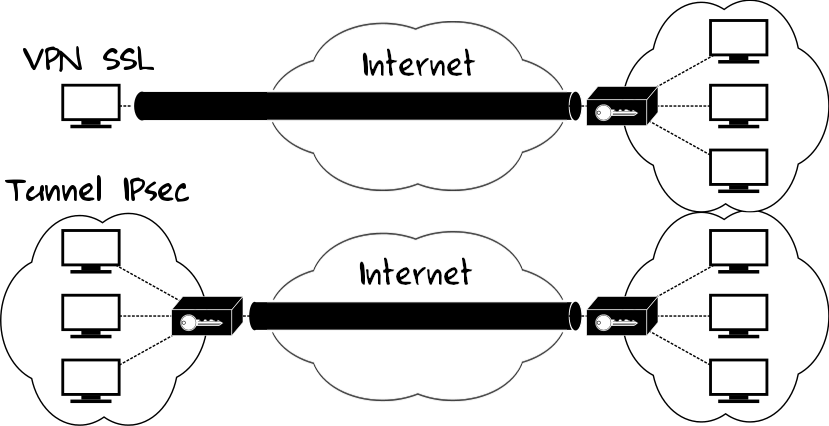
\includegraphics[width = 0.8\linewidth]{img/misc/tls-vs-ipsec.png}
    \caption{VPN TLS \textit{vs.} Tunnel IPsec --- fonctionnement typique}%
    \label{fig:misc/tls-vs-ipsec}
\end{figure}

Une fois les premières réunions passées et en parallèle des ateliers techniques,
les six pares-feux ont rapidement été commandés et livrés. Dès qu'ils ont été
réceptionnés, j'ai été chargé de tous les déballer, les installer dans la salle
de tests des bureaux de Massy et les configurer pour permettre un accès à
distance pour mon binôme de travail Silvain Bardy et moi-même. Il s'agissait ici
simplement de verser dans chaque machine la version du système d'exploitation
choisie pour ce projet et d'appliquer la même configuration partout, à quelques
petites exceptions près. De plus, j'ai dû exécuter un maximum de tests physiques
que le système d'exploitation rend disponibles pour tenter de détecter
automatiquement si une pièce de matériel était défectueuse, en particulier le
processeur, la mémoire vive, le disque dur, la carte réseau, etc\ldots{} Cela
permet de gérer ce genre de cas le plus tôt possible et directement au sein
d'\gls{ocd}. Pour chaque équipement, une petite <<Fiche de Contrôle Qualité>>
devait donc être remplie afin d'acter que les tests s'étaient bien déroulés à ce
moment-là. Un exemple d'un telle fiche est présenté en
Annexe~\ref{sec:annexes::doc-hy} (Figure~\ref{fig:doc-hy/fcq}).

\subsection{Collecte des informations et déploiement sur sites}%
\label{sub:mission::main::collec}

À partir de ce moment-là, les collaborateurs d'Hynamics devaient revenir vers
nous dès qu'ils auraient rempli d'une manière la plus exhaustive et correcte
possible un <<fichier de collecte>>. Celui-ci résume en un endroit l'ensemble
des informations que le \gls{build} ne peut pas déduire de ce qui a été discuté
en réunions et de l'architecture haut niveau précédemment conçue, c'est-à-dire
les informations métier. Cela comprend la liste des \glspl{vlan} par site, les
adresses des sous-réseaux du site et celle du pare-feu dedans, les routes
particulières, les paramètres \gls{vpn-tls}, les différents \glspl{tun-ipsec} et
surtout les règles de filtrage. Avec cette fiche bien remplie, la rédaction d'un
\gls{dsd} et l'implémentation qui s'ensuit seraient grandement facilitées et en
particulier ici, elle deviendraient presque immédiates au vu de la taille du
projet relativement petite. Un exemple d'une partie d'un fichier de collecte est
présenté en Annexe~\ref{sec:annexes::doc-hy} (Figure~\ref{fig:doc-hy/collect}).

Cependant, cette fiche ne s'est pour ainsi dire jamais vraiment remplie
complètement. En effet, il y a d'abord eu des difficultés liées simplement au
manque de compétences techniques chez les collaborateurs d'Hynamics qui créait
une difficulté au remplissage des informations demandées et un peu de confusion
à certains moments. Cela n'était pas du tout surprenant pour autant puisqu'ils
avaient bien fait appel à \gls{ocd} pour ça. Nous avons donc simplement dû gérer
cet aspect-là avec eux. Par contre, ce qui a vraiment ralenti le projet de
côté-là a surtout été les partenaires d'Hynamics qui ont mis un temps
considérable à fournir les informations nécessaires, en particulier un. Cela a
demandé de décaler dans le temps plusieurs étapes du projet à de multiples
reprises afin de pouvoir les faire correctement, mais aussi de revenir maintes
fois sur des documents et configurations qui auraient normalement dû êtres
terminés et confirmés assez tôt dans le projet. C'est pour cette raison que je
pense que le mode de travail en cascade n'était pas très adapté à ce projet:
accepter quelques cycles parmi un V aurait été assez efficace à mon avis au lieu
de décaler les choses pour toujours essayer de les faire dans l'ordre prévu
alors qu'on ne le fait en réalité déjà plus. Il y a donc eu de nombreux
va-et-vient tout au long du projet pour échanger avec le client à propos de
diverses nouvelles informations ou mises-à-jour.

C'est aussi à partir de ce moment-là que j'ai été chargé de réaliser en majeure
partie la rédaction du \acrfull{dsd}, avec l'aide et validation régulières de
mon binôme bien entendu. Le \gls{dsd} reprend notamment les informations du
fichier de collecte que nous avions reçues et qui étaient utilisables, mais
aussi certaines ajoutées comme les architectures physiques et logiques, le
détail du raccordement physique interface par interface, les routes, le
\gls{vpn-tls}, les \glspl{tun-ipsec}, la \acrfull{ha}, l'administration et la
supervision par le \gls{soc} du \gls{run}. Comme expliqué ci-dessus, le manque
d'informations arrivées à temps nous a fait rédiger une première version assez
incomplète et par la suite plusieurs itérations pour finalement assez peu de
valeur ajoutée puisque la configuration évoluait en général avant le \gls{dsd},
ce qui lui faisait alors perdre une bonne partie de son intérêt de spécification
au préalable. Cet état de fait a perduré au-delà de mon départ suite à la fin de
ma période de stage. Le plan du \gls{dsd} est présenté en
Annexe~\ref{sec:annexes::doc-hy} (Figure~\ref{fig:doc-hy/dsd}).

En parallèle, les pares-feux sont paramétrés pour simuler l'environnement de
production tout en restant dans la zone de test: nous faisions avancer la
pré-production. Cela nous a permis de mettre en place et vérifier la \gls{ha}
entre chaque paire de machines ainsi que le bon fonctionnement du \gls{vpn-tls},
au moins pour être en mesure de modifier à distance les paramètres des
pares-feux. La première configuration est ainsi assez basique, juste de quoi
permettre l'accès à distance, donc quelques utilisateurs et règles associées. Le
reste ne pourra venir qu'après puisque les informations manquaient à ce
moment-là. Les interfaces physiques et sous-interfaces \gls{vlan} sont
configurées pour que leurs adresses correspondent bien à ce qui allait être
utilisé juste après l'installation sur site et c'est ce qui a été testé. La
période de \gls{staging} s'est terminée assez rapidement puisque les choses
étaient prévues pour bien avancer peu de temps après et que peu de changements
devaient être faits, quelques jours seulement ont suffit. Après cela, j'ai dû
réaliser les opérations inverses par rapport à la précédente
Section~\ref{sub:mission::main::start}, c'est-à-dire éteindre tous les six
pares-feux, les retirer de la salle test, les remballer et les confier pour les
faire livrer au client qui s'occupera de les répartir entre les sites.
L'installation sur site se fait ensuite quelques jours plus tard, mon binôme
s'est occupé de La Défense, moi de Fontainebleau et Hynamics d'Auxerre
puisqu'ils se sentaient confiants après nous avoir observés les deux fois
précédentes et que le site est un peu plus loin des bureaux de Massy que les
deux autres.  Les déploiements sur site se sont tous bien déroulés et ont ainsi
permis l'accès à distance pour les configurer dès leur installation.

\subsection{Implémentation de la configuration}%
\label{sub:mission::main::implem}

À partir du moment où les différentes machines dont nous avions la
responsabilité directe pour la durée du projet avaient été installées, nous
avons procédé à l'évolution du \gls{dsd} et de la configuration autant que nous
le pouvions avec les informations qui nous arrivaient petit à petit, tel que
mentionné précédemment. Je vais donc reprendre ici certaines des opérations que
j'ai menées et configurations que j'ai mises en place, elles ne seront
simplement pas nécessairement présentées dans l'ordre chronologique dans lequel
elles ont effectivement été appliquées.

La première étape aura été de revoir les interfaces qui sont présentées en
Figure~\ref{fig:fgt-auxr/interfaces}. En effet, de nouvelles informations nous
étaient parvenues et nous devions ajouter de nouvelles sous-interfaces
\gls{vlan} pour les partenaires qui avaient initialement été prévus pour avoir
leur machines dans le sous-réseau dédié à Hynamics. De plus, certaines des
interfaces représentant les \glspl{tun-ipsec} ont dû être modifiées pour
recevoir une adresse spécifique au tunnel afin de gérer correctement le
\gls{bgp}. Enfin, des droits supplémentaires autorisés sur les interfaces
publiques, tels la capacité d'effectuer un \textit{ping} ou d'administrer le
pare-feu en HTTPS ou SSH, avaient été maintenus pour garder un accès de secours
en attendant la validation du bon fonctionnement du \gls{vpn-tls}. Ils ont été
retirés une fois tout bien configuré.

\begin{figure}[h!]
    \centering
    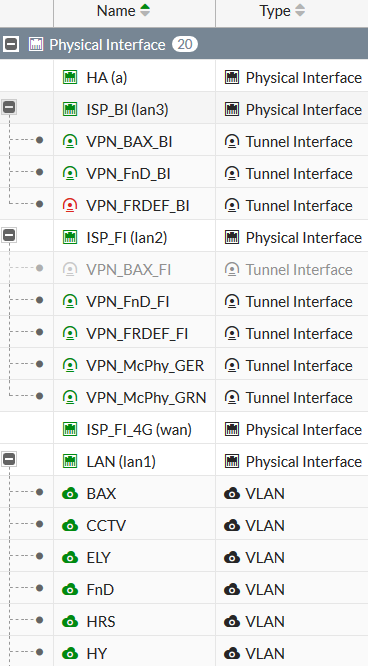
\includegraphics[width = 0.5\linewidth]{img/fgt-auxr/interfaces.png}
    \caption{Interfaces du pare-feu d'Auxerre}%
    \label{fig:fgt-auxr/interfaces}
\end{figure}

Ensuite, les routes statiques, montrées en Figure~\ref{fig:fgt-auxr/routes}, ont
eu besoin d'être changées régulièrement pour prendre en compte les nouveautés au
niveau de l'architecture. En particulier, les \glspl{tun-ipsec} entre La Défense
et les sites de production, mais aussi ceux avec les partenaires qui étaient
souvent changés en fonction de la recherche de solution avec eux. Les trois
premières routes n'ont cependant jamais changé puisqu'il s'agit des routes par
défaut redirigeant vers les routeurs des trois liens Internet locaux. Celles
concernant les \glspl{tun-ipsec} inter-sites n'ont pas non plus beaucoup changé
une fois configurées et vérifiées.

\begin{figure}[h!]
    \centering
    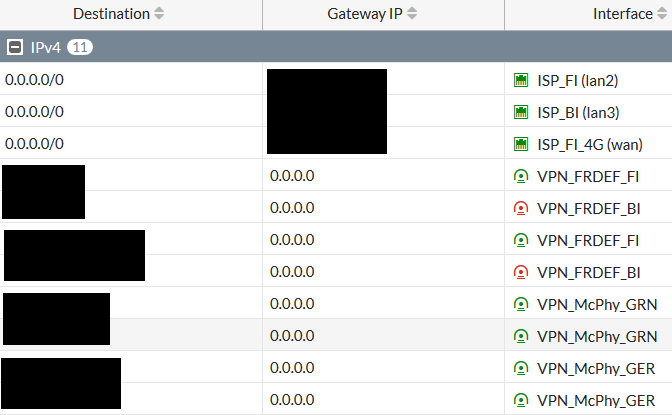
\includegraphics[width = 0.8\linewidth]{img/fgt-auxr/routes.png}
    \caption{Routes statiques du site d'Auxerre}%
    \label{fig:fgt-auxr/routes}
\end{figure}
\FloatBarrier{}

Un \gls{tun-ipsec} est configuré sous \acrlong{fgt} avec les morceaux de
configuration suivants:

\begin{itemize}
    \item Une <<phase 1>> qui paramètre le comportement d'\gls{ike} et
        l'initialisation de la connexion, avec les options principales suivantes:

    \begin{itemize}
        \item \texttt{interface}: l'interface sur laquelle écouter et
            communiquer;
        \item \texttt{remote-gw}: l'hôte distant auquel se connecter;
        \item \texttt{proposal}: la liste de couples algorithme de chiffrement /
            algorithme de hachage à proposer au correspondant distant;
        \item \texttt{psksecret}: le secret pré-partagé.
    \end{itemize}

    \item Une ou plusieurs <<phases 2>> qui paramètrent le comportement
        d'\gls{esp} et la communication effective, avec les options principales
        suivantes:

    \begin{itemize}
        \item \texttt{phase1name}: l'identifiant de la phase 1 à utiliser;
        \item \texttt{proposal}: la liste de couples algorithme de chiffrement /
            algorithme de hachage à proposer au correspondant distant;
        \item \texttt{dhgrp}: le groupe Diffie-Hellmann à utiliser pour
            construire le secret commun avec le correspondant distant;
        \item \texttt{src-subnet}: le réseau local dont les paquets sont à faire
            passer au travers du tunnel vers le correspondant;
        \item \texttt{dst-subnet}: le réseau distant dont les paquets sont à
            recevoir depuis le correspondant.
    \end{itemize}
\end{itemize}

La configuration des \glspl{tun-ipsec} a d'abord commencée avec ceux reliant les
sites de production de Fontainebleau et d'Auxerre au central de La Défense dans
le but de permettre la communication entre les pares-feux et le \gls{fmg} et le
\gls{faz}. Pour assurer un service le plus constant possible, l'architecture
prévoyait dès le départ d'avoir une redondance sur ces tunnels. Elle est
réalisée entre sites grâce à l'option \texttt{monitor} des \acrlongpl{fgt}.
Cette option permet de définir un tunnel principal et un tunnel secondaire et
ainsi de n'avoir qu'un seul tunnel connecté à la fois: le tunnel secondaire qui
a l'option configurée surveille le tunnel principal et s'il arrête de
fonctionner, le secondaire ne va alors chercher à se connecter au correspondant
qu'à partir de ce moment-là, sinon il reste inactif; lorsque le tunnel principal
revient à la vie, il se connecte alors et le secondaire s'éteint. Un exemple de
phase 1 utilisant ce genre de fonctionnalité est mis à disposition en
Figure~\ref{fig:fgt-auxr/ipsec-phase1}. Le tunnel primaire passe par le lien
\gls{fi} et le secondaire par le \gls{bi}.

\begin{figure}[h!]
    \centering
    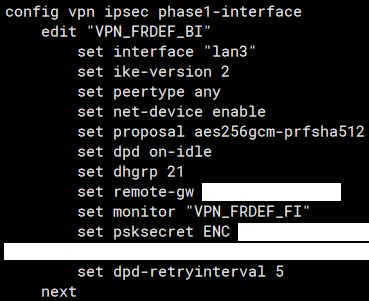
\includegraphics[width = 0.6\linewidth]{img/fgt-auxr/ipsec-phase1.png}
    \caption{Extrait d'une phase 1 inter-sites entre Auxerre et La Défense}%
    \label{fig:fgt-auxr/ipsec-phase1}
\end{figure}

En général, il est possible de n'avoir qu'une seule phase 2 par phase 1 dès lors
qu'un seul réseau est utilisé des deux côtés du tunnel. Cependant, si un second
réseau a besoin de passer à un des deux côtés, il faut ajouter une nouvelle
phase 2 correspondante: chaque paire de sous-réseaux devant pouvoir communiquer
pour une phase 1 donnée doit avoir sa phase 2 dédiée. Par exemple, le partenaire
McPhy a plusieurs sites distants et plusieurs sous-réseaux distants par site, on
peut en voir une conséquence sur les routes statiques montrées en
Figure~\ref{fig:fgt-auxr/routes}. Les partenaires FillinDrive et BaxEnergy ont
eux leurs infrastructures distantes hébergées chez des fournisseurs de
\textit{cloud} qui ne permettent pas de configuration similaire à ce que fait
l'option \texttt{monitor} de \acrlong{fgt}, mais seulement une bascule au niveau
routage grâce à \gls{bgp}, les deux tunnels restent alors actifs à tout moment.
Pour que le \gls{bgp} puisse s'établir entre les deux routeurs reliés par les
\glspl{tun-ipsec}, il faut donc configurer une seconde phase 2 dédiée à la
communication purement \gls{bgp} et locale au lien. Un exemple d'une telle
configuration est présentée en Figure~\ref{fig:fgt-auxr/ipsec-phase2}.

\begin{figure}[h!]
    \centering
    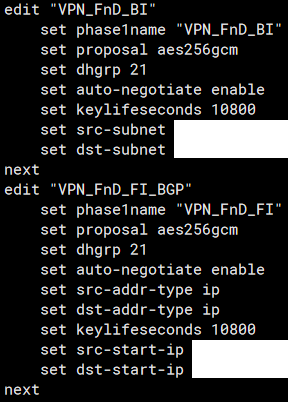
\includegraphics[width = 0.5\linewidth]{img/fgt-auxr/ipsec-phase2.png}
    \caption{Extrait de phases 2 de FillinDrive sur le site d'Auxerre}%
    \label{fig:fgt-auxr/ipsec-phase2}
\end{figure}
\FloatBarrier{}

Deux partenaires ont leurs infrastructures hébergées sur du \textit{cloud} qui
ne permettent pas une redondance active-passive avec deux tunnels où le
secondaire est éteint tant que le primaire fonctionne. Il a donc fallu pour ces
partenaires mettre en place une redondance active-active avec une bascule
assurée par \gls{bgp}. Une configuration équivalente avait été essayée avec du
routage statique, mais ne fonctionnait pas car ces plates-formes ne permettent
en général pas de configurer des routes statiques ayant des priorités définies.

\acrfull{bgp} est un protocole standardisé de passerelle externe conçu pour
échanger des informations de routage et de disponibilité entre systèmes
autonomes (\gls{as}) de l'Internet. C'est un protocole de routage à vecteur de
chemin puisque les décisions de routage sont effectuées sur la base de chemins,
politiques réseaux ou ensembles de règles configurés par un administrateur
réseau. Il permet ainsi de contrôler depuis un niveau assez haut les flux de
l'Internet, ce qui est parfois nécessaire pour des raisons simplement
géopolitiques. Un \gls{as} est une collection de préfixes de routage IP sous le
contrôle d'un ou plusieurs opérateurs réseau au nom d'une seule entité ou
domaine administratif et qui présente à l'Internet une politique de routage
commune et clairement définie. Un tel système autonome est identifié par un
\gls{asn}, un nombre entier originellement sur deux octets, maintenant quatre.
C'est cet identifiant qui sert à configurer les politiques \gls{bgp}.

La Figure~\ref{fig:fgt-auxr/bgp-neighbors} montre la configuration \gls{bgp}
pour le partenaire FillinDrive. La section \texttt{config router bgp} est
valable pour tous les voisins \gls{bgp}. Elle comporte notamment l'option
\texttt{as} qui définit l'\gls{asn} que présente le routeur. Ces voisins sont
renseignés dans la sous-section \texttt{config neighbor}. Chaque entrée a pour
nom l'adresse du routeur distant et a pour paramètre principal
\texttt{remote-as} l'\gls{asn} qu'il présente. On remarquera qu'entre les deux
entrées qui configurent chacune le routage pour un des deux tunnels en
redondance, il y a assez peu de différences, une est l'option \texttt{weight}:
le poids des routes associées. Cela permet de définir des priorités entre les
chemins équivalents, c'est-à-dire ici depuis l'\gls{as} local vers l'\gls{as}
distant. Le poids de \texttt{100} est appliqué au tunnel passant par le lien
\gls{fi} pour lui donner une priorité plus importante ($100 > 10$) et en faire
ainsi le tunnel primaire.

\begin{figure}[h!]
    \centering
    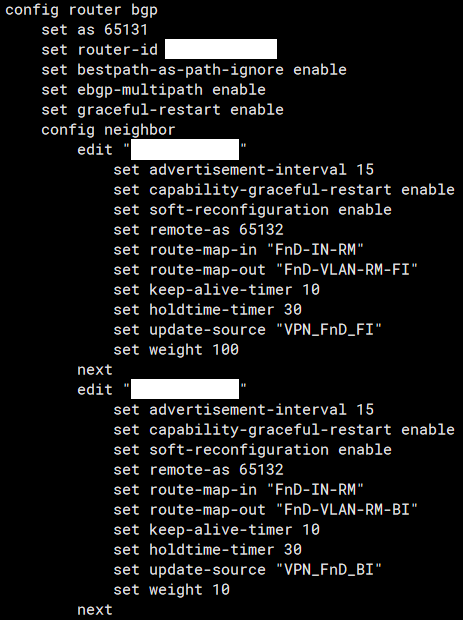
\includegraphics[width = 0.6\linewidth]{img/fgt-auxr/bgp-neighbors.png}
    \caption{%
        Extrait de la configuration \gls{bgp} du site d'Auxerre avec les voisins
        pour FillinDrive%
    }%
    \label{fig:fgt-auxr/bgp-neighbors}
\end{figure}

La Figure~\ref{fig:fgt-auxr/bgp-nets} montre comment sont configurés les réseaux
distribués aux voisins. Chaque entrée comporte une option principale
\texttt{prefix} qui donne ce par quoi doit commencer une adresse pour être
considérée comme faisant partie du réseau. Il ne peut donc pas y avoir toutes
les possibilités fournies par les masques IP qui ne sont pas eux-mêmes de
simples préfixes. Les réseaux ainsi définis sont cependant distribués à tous les
voisins, ce qui n'est pas idéal lorsque plusieurs \gls{as} y sont reliés.

\begin{figure}[h!]
    \centering
    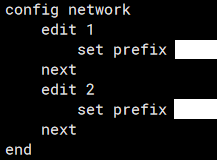
\includegraphics[width = 0.4\linewidth]{img/fgt-auxr/bgp-nets.png}
    \caption{Réseaux distribués par \gls{bgp} sur le site d'Auxerre}%
    \label{fig:fgt-auxr/bgp-nets}
\end{figure}

Les \acrlongpl{fgt} mettent alors à disposition la notion de liste d'accès
(\textit{access list} en anglais) qui permet de configurer un filtre d'adresses.
La Figure~\ref{fig:fgt-auxr/acl} en montre ainsi deux: une pour chaque
partenaire concerné --- les préfixes sont donc bien différents.

\begin{figure}[h!]
    \centering
    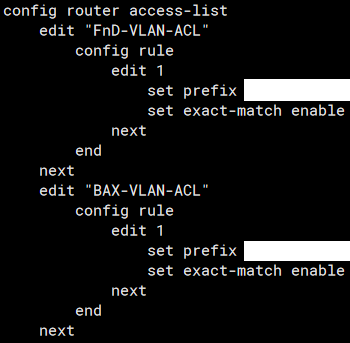
\includegraphics[width = 0.6\linewidth]{img/fgt-auxr/acl.png}
    \caption{%
        Filtres d'adresses pour le \gls{bgp} de FillinDrive et BaxEnergy sur
        Auxerre%
    }%
    \label{fig:fgt-auxr/acl}
\end{figure}

Pour pouvoir être appliquée à un voisin, il faut que cette liste d'accès soit
incluse dans une <<carte de routage>> (\textit{route map} en anglais) qui permet
de décrire un ensemble de règles qui ont chacune une liste d'accès comme filtre
d'adresse et un certain nombre d'autres options qui configurent les paramètres
de la routes dynamique à créer en cas de correspondance avec le filtre. La
différence entre les deux entrées montrées en
Figure~\ref{fig:fgt-auxr/route-maps} réside en l'option \texttt{set-metric}:
elle configure la priorité à envoyer à l'\gls{as} distant afin qu'il l'applique
sur ses routes dynamiques de sa table. Elle est cette fois-ci inverse par
rapport au poids, \texttt{10} est donc plus prioritaire que \texttt{100} et est
alors utilisée pour le lien primaire \gls{fi}. Une fois appliquées aux
configurations des voisins, ces \textit{route maps} constituent le dernier
paramètre nécessaire pour mettre en place l'architecture souhaitée.

\begin{figure}[h!]
    \centering
    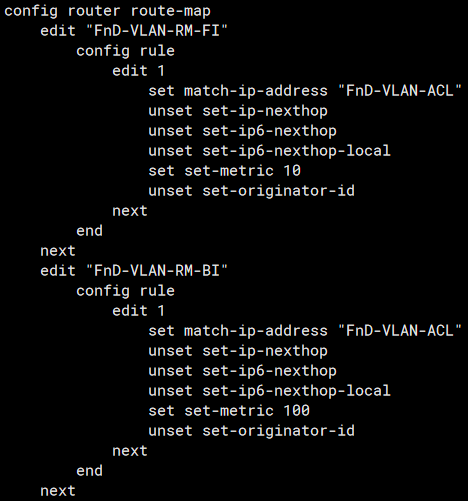
\includegraphics[width = 0.7\linewidth]{img/fgt-auxr/route-maps.png}
    \caption{Associations de routes \gls{bgp} de FillinDrive sur Auxerre}%
    \label{fig:fgt-auxr/route-maps}
\end{figure}
\FloatBarrier{}

Après avoir configuré les pares-feux avec des paramètres basiques, je les ai
reliés au \acrlong{fmg} et au \acrlong{faz} situés sur le site central de La
Défense. \acrfull{fmg} est une solution de gestion centralisée des produits
Fortinet, en particulier les pares-feux. Elle permet notamment par rapport à ces
derniers de stocker certains objets dont dépend la majeure partie de leurs
configurations tels que les adresses (Figure~\ref{fig:fmg/addresses}), les
services (Figure~\ref{fig:fmg/services}) et les interfaces normalisées
(Figure~\ref{fig:fmg/interfaces}).

\begin{figure}[h!]
    \centering
    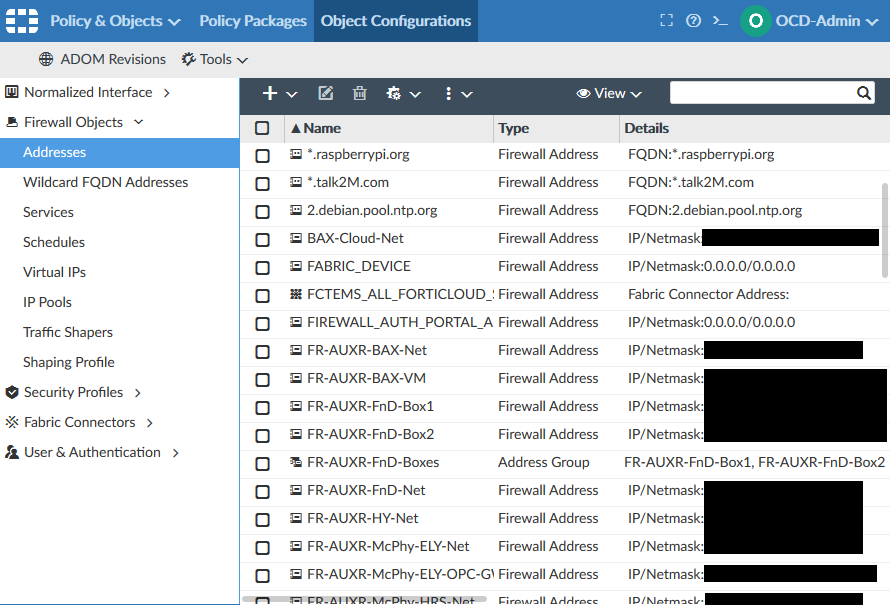
\includegraphics[width = \linewidth]{img/fmg/addresses.png}
    \caption{Adresses configurées centralement sur le \acrlong{fmg}}%
    \label{fig:fmg/addresses}
\end{figure}

\begin{figure}[h!]
    \centering
    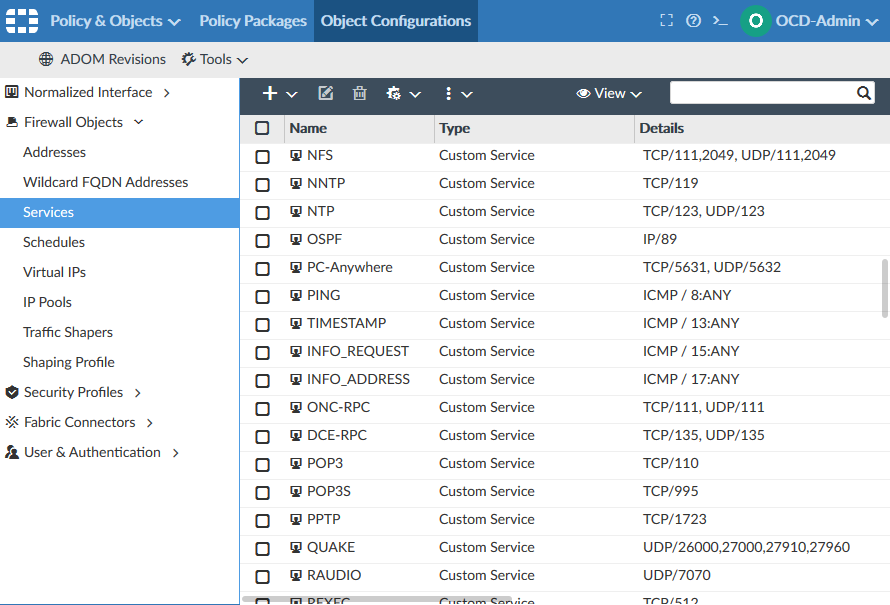
\includegraphics[width = \linewidth]{img/fmg/services.png}
    \caption{Services configurés centralement sur le \acrlong{fmg}}%
    \label{fig:fmg/services}
\end{figure}

Une interface normalisée est une interface utilisable dans les règles de
filtrage d'un \gls{pp} mais qui regroupe en réalité un ensemble de <<vraies>>
interfaces, une pour chaque machine effective.  La vraie interface est
sélectionnée quand le \gls{pp} est appliqué à une certaine machine. Cela permet
donc de créer des règles valables pour de nombreuses machines sans pour autant
devoir se répéter.

\begin{figure}[h!]
    \centering
    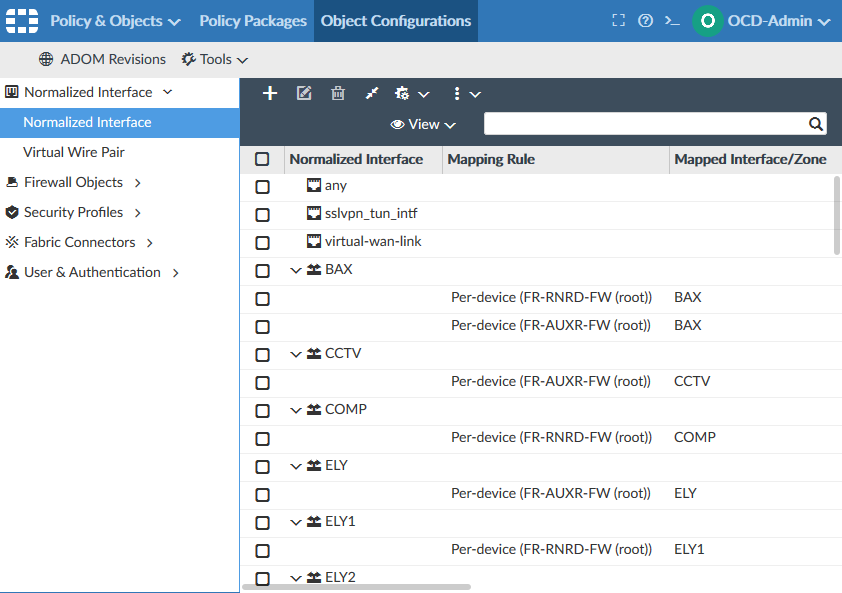
\includegraphics[width = \linewidth]{img/fmg/interfaces.png}
    \caption{Interfaces normalisées sur le \acrlong{fmg}}%
    \label{fig:fmg/interfaces}
\end{figure}

Le \acrlong{fmg} introduit aussi la notion de \gls{pp}. Un \gls{pp} est l'unité
de configuration qui comporte principalement les règles de filtrage des
différents pares-feux gérés par le \gls{fmg}, mais aussi tous les objets dont
elles dépendent tels qu'adresses, interfaces, services, utilisateurs ou groupe
d'utilisateurs, et qui peut être appliqué à un ou plusieurs pares-feux. Nous
avons dans notre cas fait un \gls{pp} par pare-feu car les configurations
n'avaient que trop peu de similitudes pour réaliser une seule suite de règles
communes. La Figure~\ref{fig:fmg/policy-packages} en montre un exemple.
L'intérêt du \acrlong{fmg} se fait remarquer surtout lorsqu'un objet commun à
plusieurs \glspl{pp} est modifié. Si par exemple un utilisateur est ajouté à un
groupe qui est utilisé dans certaines règles de plusieurs \glspl{pp}, le
\acrlong{fmg} va alors considérer que tous les \glspl{pp} concernés ont été
modifiés et qu'il faut les envoyer aux machines qu'ils paramètrent de sorte
qu'elles soient mises à jour. On peut faire se dernier point de manière
parallélisée et l'utilisateur est ainsi ajouté à tous les pares-feux bien plus
rapidement que s'il fallait le configurer manuellement sur chacun d'entre-eux.

\begin{figure}[h!]
    \centering
    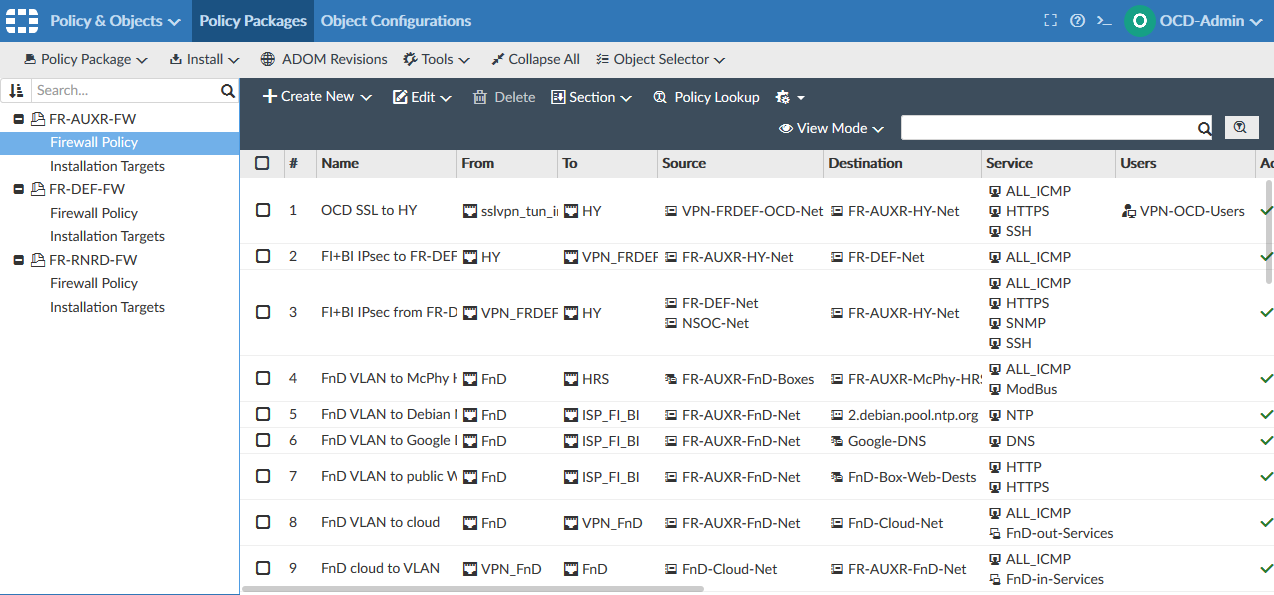
\includegraphics[width = \linewidth]{img/fmg/policy-packages.png}
    \caption{\Glspl{pp} du \acrlong{fmg}}%
    \label{fig:fmg/policy-packages}
\end{figure}
\FloatBarrier{}

J'ai par la suite été chargé de configurer les accès en \gls{vpn-tls} pour les
collaborateurs d'Hynamics et de leurs partenaires. Cette opération est en grande
partie faisable centralement depuis le \acrlong{fmg}. Il s'agit principalement
de créer des associations de groupes d'utilisateurs à leurs droits accordés en
termes de connexion et routes communiquées (Figure~\ref{fig:fmg/ssl-mappings}).
Il faut ensuite bien évidemment aussi paramétrer de nouvelles règles de filtrage
permettant la communication en \gls{vpn-tls} des utilisateurs avec les
ressources de leur sous-réseau dédié.

\begin{figure}[h!]
    \centering
    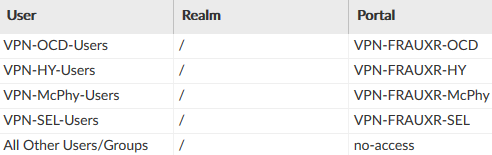
\includegraphics[width = 0.8\linewidth]{img/fmg/ssl-mappings.png}
    \caption{%
        Associations des portails aux groupes d'utilisateurs pour le
        \gls{vpn-tls} sous \acrlong{fmg}%
    }%
    \label{fig:fmg/ssl-mappings}
\end{figure}

Fortinet utilise la notion de <<portail SSL>>, dont un exemple est présenté en
Figure~\ref{fig:fmg/ssl-portal}, afin de décrire ces droits spécifiques et
paramètres de connexion. Les trois options importantes pour l'utilisation que
nous en faisions étaient le \textit{split tunneling}, les routes et les réseaux
sources. Le \textit{split tunneling} consiste à ne pas rediriger tout le trafic
au travers du tunnel \gls{vpn-tls}, mais uniquement celui à destination de ce
qui est mis à disposition par la passerelle. Les routes sont les sous-réseaux
accessibles depuis la passerelle et qui sont communiqués au client se connectant
afin qu'il les enregistre dans sa table de routage. Les réseaux sources
(\textit{source IP pools}) déterminent quelles plages d'adresses vont être
utilisées pour y allouer dynamiquement des adresses sources locales pour les
clients se connectant.

\begin{figure}[h!]
    \centering
    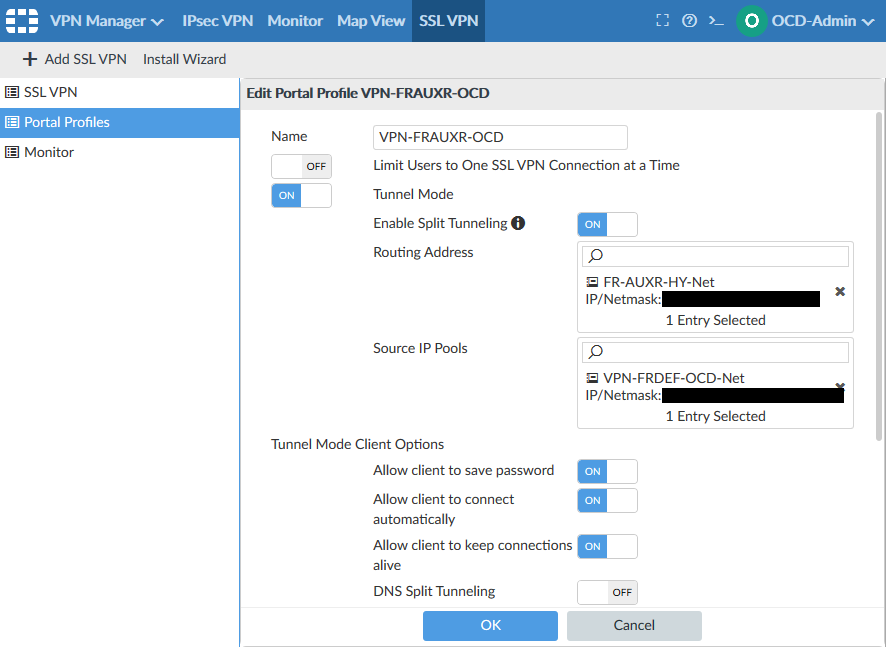
\includegraphics[width = \linewidth]{img/fmg/ssl-portal.png}
    \caption{Portail \gls{vpn-tls} sous \acrlong{fmg}}%
    \label{fig:fmg/ssl-portal}
\end{figure}

\FloatBarrier{}
\subsection{Mise en place des tests et migration}%
\label{sub:mission::main::tests}

Une fois l'implémentation effectuée, il s'agit ensuite de préparer puis réaliser
une suite de tests afin de confirmer que tout fonctionne comme prévu. Nous avons
donc préparé un \acrfull{dtv} par site en parallèle de la fin de
l'implémentation. Un tel \gls{dtv} est relu, corrigé puis validé par le client
avant d'effectuer les tests en séance lors d'une \acrfull{vabf}. Un exemple de
fiche de tests complétée est présenté en Annexe~\ref{sec:annexes::doc-hy}
(Figure~\ref{fig:doc-hy/dtv}).

Nous avons d'abord réalisé la \gls{vabf} pour le site de La Défense, tout
simplement car il s'agissait du plus facile à implémenter et à tester. Le site
de Fontainebleau n'a malheureusement pas pu être avancé jusqu'à ce point car un
problème d'ordre industriel y était survenu, ce qui l'a rendu momentanément
inexploitable. Il n'était donc plus pertinent de chercher à le compléter puisque
seulement très peu d'informations utilisables nous étaient transmises à son
sujet. Son implémentation n'a donc été que très partielle et aucune \gls{vabf}
associée n'a été effectuée pendant mon stage: les choses de côté-là ont été
décalées à au moins un mois après la fin de celui-ci. Le seul site de production
qui a été presque entièrement terminé puis validé en \gls{vabf} a donc été celui
d'Auxerre.

Cette \gls{vabf} avait été organisée pour être effectuée sur une journée entière
en réalisant une séance par partenaire, en commençant par Hynamics. Cette
première séance nous a permis d'exécuter la majeure partie des tests prévus dans
le \gls{dtv} du site et ainsi de vérifier notamment la bonne communication du
\acrlong{fgt} avec le \acrlong{fmg} et le \acrlong{faz}, le bon fonctionnement
de la redondance physique en cas de débranchement (\textit{i.e.} perte) d'un des
deux pares-feux de la paire, de même lorsque l'un des liens Internet ne
fonctionne plus pour un des deux pares-feux, \ldots{} Les opérations que cherche
à réaliser le \gls{run} ont aussi été vérifiées en leur présence, telles que la
supervision, la sauvegardes des configurations et l'intégration dans la base de
données de gestion automatisée des équipements. Viennent ensuite les tests
d'ordre plutôt applicatif, à commencer pour Hynamics par leur accès en
\gls{vpn-tls}.

Ceux-ci se sont rapidement heurtés à un problème simple mais important: le
commutateur central du site n'était pas administrable et ne pouvait en
particulier pas gérer les \glspl{vlan}. Toute communication effectuée à
distance, c'est-à-dire sans passer directement par un unique câble, et tentée
avec un équipement autre que le pare-feu ne pouvait donc pas fonctionner. Cela a
eu un impact immédiat: très peu de tests applicatifs ont pu être réalisés, que
ça soit avec Hynamics, mais surtout avec les partenaires pendant le reste de la
journée. Cet oubli de notre part est en quelque sorte double: les \gls{presales}
n'avaient pas mentionné ce point important en début de projet et nous de notre
côté \gls{build} leur avions fait confiance pour l'avoir justement précisé sans
que nous le redemandions pour autant car cette partie purement locale ne faisait
pas partie des choses dont nous devions nous préoccuper dans le cadre du projet
et relèvait plus de la responsabilité du client et de ses partenaires.  Un
nouveau commutateur a donc dû être acheté quelque peu dans l'urgence le jour
même pour ensuite être configuré le soir et le lendemain.

Le commutateur acheté était un Dell mais exécutant Cisco IOS~\cite{cisco-ios}.
La configuration à implémenter restait relativement simple: il s'agissait
d'ajouter quelques \glspl{vlan} (Figure~\ref{fig:sw-auxr/vlans}) au moins un par
partenaire et ensuite de paramétrer les interfaces physiques reliées aux divers
équipements du site. On a par exemple dédiées aux deux pares-feux de la paire en
Figure~\ref{fig:sw-auxr/fw-ifs} et celles pour le serveur ESXi en
Figure~\ref{fig:sw-auxr/esxi-ifs}. Plus précisément, ce dernier n'en a en
réalité qu'une qui lui est affectée, l'autre permet de l'administrer si jamais
une personne est présente sur site. En effet, ce serveur expose une interface
d'administration Web que nous avons configurée pour communiquer sur le
\gls{vlan} \texttt{10}, c'est-à-dire celui d'Hynamics. Il héberge surtout une
machine virtuelle pour le partenaire BaxEnergy qui doit donc être dans son
propre \gls{vlan}, le numéro \texttt{70}. D'où la configuration présentée de la
première interface. Pour la seconde, il s'agit simplement de pouvoir se mettre
dans le \gls{vlan} d'Hynamics si on est physiquement sur site mais sans pour
autant devoir configurer le système d'exploitation de son poste pour avoir une
interface \gls{vlan} puisque le commutateur est là en mode \texttt{access}.
Celui-ci s'occupe d'ajouter à chaque trame Ethernet l'en-tête IEEE 802.1q avec
un identifiant de \gls{vlan} fixé, ici le \texttt{10}. L'autre mode utilisé dans
le reste des interfaces présentées est le \texttt{trunk} qui permet de
rassembler en un lien des trames étant étiquetées avec des identifiants
\gls{vlan} faisant partie d'une liste configurée.

\begin{figure}[h!]
    \centering
    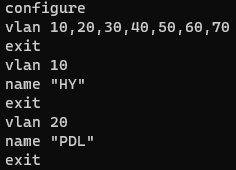
\includegraphics[width = 0.4\linewidth]{img/sw-auxr/vlans.png}
    \caption{Configuration des \glspl{vlan} du commutateur central d'Auxerre}%
    \label{fig:sw-auxr/vlans}
\end{figure}

\begin{figure}[h!]
    \centering
    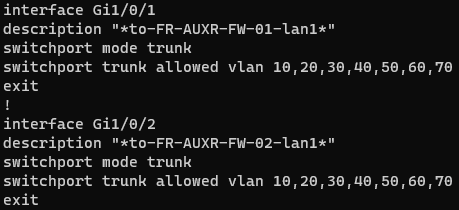
\includegraphics[width = 0.7\linewidth]{img/sw-auxr/fw-ifs.png}
    \caption{%
        Configuration des interfaces du commutateur central connectées au
        pare-feu d'Auxerre%
    }%
    \label{fig:sw-auxr/fw-ifs}
\end{figure}

\begin{figure}[h!]
    \centering
    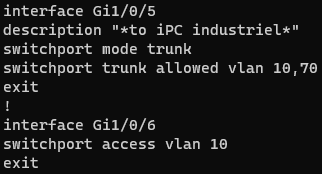
\includegraphics[width = 0.5\linewidth]{img/sw-auxr/esxi-ifs.png}
    \caption{%
        Configuration des interfaces du commutateur central dédiées au serveur
        ESXi (hyperviseur) d'Auxerre%
    }%
    \label{fig:sw-auxr/esxi-ifs}
\end{figure}
\FloatBarrier{}

Nous avons tout de même été en mesure de réaliser de nombreuses opérations lors
de la journée initialement dédiée à la \gls{vabf} entière. La plupart des
partenaires n'avaient malheureusement pas terminé la configuration de leur côté
alors que nous leur avions explicitement demandé de le faire en avance afin
d'éviter de perdre du temps inutilement et de potentiellement devoir remettre
les choses aux jours suivants, ce qui a dû finalement être fait pour plusieurs
raisons, le mauvais commutateur entre autres. Nous avons donc dû revoir avec eux
les paramètres des \glspl{tun-ipsec} que nous leur avions fait parvenir les
jours ou semaines précédents, les aider à les appliquer dans leurs outils
respectifs et résoudre les problèmes apparaissant au fur et à mesure de la
séance. Le \gls{vpn-tls} n'a pas particulièrement posé de souci puisque les
réglages étaient surtout de notre côté et l'utilisation du leur se repose sur le
FortiClient utilisé. Un exemple de fiche rassemblant les paramètres de tunnels
et communiquée à un des partenaires est présentée en
Annexe~\ref{sec:annexes::doc-hy} (Figure~\ref{fig:doc-hy/ipsec-tun}).

Il y a cependant eu un problème avec le partenaire BaxEnergy qui est hébergé
chez Microsoft Azure qui nous a demandé pas mal de temps à investiguer. En
effet, ils avaient commencé avec une configuration active-passive car plus
simple et n'utilisant qu'une seule passerelle publique.  Seulement, la
redondance ne fonctionnait pas comme souhaité car les routes statiques
n'acceptaient pas de priorité et la bascule ne permettait donc pas de revenir au
tunnel primaire dès lors qu'il revenait à la vie. Il a donc fallu passer à une
configuration active-active et assurer la bascule avec \gls{bgp} de manière
similaire à ce qui était déjà fait avec l'autre partenaire FillinDrive.
Malheureusement, même après avoir revu maintes fois les paramètres appliqués et
essayé de nombreuses combinaisons, nous n'avons pas réussi à le faire
fonctionner correctement. Plus précisément, les deux tunnels se montaient sans
erreur, tandis que le \gls{bgp} fonctionnait sur le tunnel primaire mais pas au
travers du secondaire: il semblait être refusé immédiatement du coté d'Azure. Le
partenaire BaxEnergy a alors dû se résigner à ouvrir un ticket de support auprès
de Microsoft afin d'élucider le problème car tout semblait pointer vers une
erreur de leur côté.

\FloatBarrier{}
\subsection{Transferts de connaissances}%
\label{sub:mission::main::trans}

À la suite de la fin de l'implémentation, nous avons avec mon binôme \gls{build}
du projet dû effectuer quelques transferts de connaissances pour assurer la
bonne continuation des opérations après notre intervention. Cela concernait en
un premier temps l'ingénieur \gls{run} chargé du suivi régulier du parc ainsi
installé et des changements de configuration à effectuer dans le futur. Il a
fallu aussi le faire à la fin de mon stage avec une stagiaire \gls{build}
récemment arrivée puisque les quelques problèmes mentionnés précédemment avaient
encore une fois décalé les étapes initialement prévues. Il s'agissait donc de
présenter le projet d'un point de vue assez global puis d'entrer dans plus de
détails concernant directement la personne en question afin qu'elle ait à
l'esprit les éléments qu'elle aillait utiliser régulièrement.


\section{Relations humaines et management}%
\label{sec:mission::rhm}

Comme pour de très nombreuses entreprises, la gestion des conséquences de la
pandémie a été particulièrement complexe. Un des effets immédiats a été le
télétravail presque permanent, les relations humaines directes ont donc été très
restreintes. Le nombre de personnes présentes dans les bureaux ne dépassait en
général pas cinq par étage pour des équipes pourtant bien plus grandes. Bien
évidemment, toute opération nécessairement physique demandait une présence
physique. Cela inclut notamment les actions menées sur la salle de test en début
de stage et les déploiements pour le projet Hynamics.

La majeure partie du stage s'est donc effectuée en télétravail car, même si
autorisé de temps à autre, il n'y avait en réalité que très peu d'intérêt à se
rendre aux bureaux puisque les gens avec qui je travaillais directement n'y
étaient pas régulièrement. L'ensemble des communications fréquentes et réunions
se sont alors faites avec Microsoft Teams. Cette organisation est relativement
efficace sur certains points pratiques, comme la rapidité d'échange
d'informations déjà numérisées ou le passage d'une réunion à l'autre en très peu
de temps. Cela nous permet notamment d'économiser un temps considérable en
trajets. Elle n'est cependant, je trouve, pas aussi efficace ou en tout cas
agréable sur d'autres points. Je pense par exemple au besoin d'aide régulier en
tant que débutant sur de nombreux sujets: être physiquement à côté d'une équipe
entière favorise à mon avis le sentiment de liberté d'approche dans ce genre de
situations. Cela augmente aussi la cohésion d'équipe par interaction régulière.

Certains moments de la semaines ont été dédiés à des activités purement d'équipe
pour tenter de pallier ces effets secondaires du télétravail quotidien. Il y
avait par exemple une réunion hebdomadaire d'une heure le jeudi soir prévue pour
être un moment d'interaction détendue et d'échange sur les dernières nouvelles
de chacun afin que les membres de l'équipe soient au moins un peu au courant de
ce qui est en cours en terme de projets client, internes, nouveaux sujets,
formations, \ldots{} Deux heures étaient aussi réservées le vendredi matin pour
diverses formations internes. Cela permet de monter en compétences sur de
nouveaux sujets que l'on a pas encore été en mesure d'aborder, mais aussi de
suivre les dernières nouveautés relatives aux quelques produits que l'on a déjà
pu pratiquer. En dehors de ces moments-là, il n'y avait cependant qu'assez peu
d'interactions liées directement au travail: les équipes projet sont en général
assez petites, beaucoup de choses sont faites indépendamment des autres
ingénieurs de l'équipe totale. C'est un aspect de l'\gls{integ} que je trouve un
peu dommage, je ne ressentais pas autant de cohésion au sein de l'équipe entière
que je ne l'aurais initialement imaginé.

Le mode de travail est, comme mentionné précédemment, principalement organisé
autour de projets client. C'est alors surtout au chef de projet d'assurer son
bon déroulement et donc le management direct de l'équipe projet associée. Le
management au niveau de l'équipe d'\gls{integ} globale concerne plutôt les
réaffectations d'un projet à un autre.

\chapter{Responsabilité sociétale des entreprises}%
\label{cha:rse}

La \gls{rse} désigne la responsabilité des entreprises dans les enjeux sociaux,
environnementaux, économiques et éthiques. Cela comprend notamment les questions
de développement durable où comment les activités doivent être viables sur le
long terme que ce soit socialement ou écologiquement. La Santé et Sécurité au
Travail fait également parti de la \gls{rse} sur ses composantes économiques et
éthiques.

\section{Social}%
\label{sec:rse::social}

\acrlong{ocd} met en place une série de mesures pour lutter contre les
discriminations. Il s'agit d'encourager la diversité au sein de l'entreprise et
de l'industrie.  De plus, les salaires sont identiques pour tout le monde au
niveau junior, cela ne dépend que du niveau hiérarchique. Les grilles salariales
sont ainsi transparentes, fixes et indépendantes d'une quelconque négociation.

\gls{ocd} prend en particulier très au sérieux la diversité et l'égalité
homme-femme. Une de leurs priorités est de favoriser la féminisation des métiers
techniques et du numérique dans lesquels les femmes sont sous-représentées
actuellement. 24\% des managers sont actuellement des femmes. Un objectif
annoncé est d'atteindre d'ici 2025 25\% de femmes dans les métiers techniques et
du numérique et 35\% de femmes dans les postes à responsabilité, l'égalité
salariale entre les femmes et les hommes à situation comparable.

L'entreprise et le groupe mettent notamment en place des formations ouvertes aux
professionnels et aux étudiants. <<Orange Campus>> propose par exemple des
formations professionnelles ouvertes aux étudiants comme aux professionnels,
orientées sur les expertises numériques: data \& IA, cybersécurité, management,
\textit{soft skills}. Dans le cadre d'Orange Campus, <<Orange Cyberdéfense
Academy>> est un programme unique combinant un poste en CDI avec un cursus
diplômant bac+5.  <<École de la Data>> est aussi disponible: une école dédiée
aux nouveaux métiers de \textit{Data Engineer} et \textit{Data Scientist}, et
qui recrute aujourd'hui près de 40\% de femmes.

\section{Environnement}%
\label{sec:rse::env}

\gls{ocd} essaie d'inclure de plus en plus certains aspects environnementaux
dans leurs démarches régulières. Le groupe Orange a par exemple lancé en 2020 le
programme \textit{Green Act}, un programme d'accélération pour encourager
l'ensemble de ses filiales et de ses parties prenantes à intégrer les enjeux
environnementaux au cœur de leurs processus et de leurs activités.
\acrlong{obs} possède ainsi deux centres de données <<verts>>, 50\% des routeurs
récupérés sont reconditionnés et réutilisés, 46\% des bureaux sont certifiés ISO
14 001 et 16\% d'énergie renouvelable est utilisée dans sa consommation. Orange
est noté 77\up{ième} sur 100 parmi le premier pourcent des entreprises les plus
écoresponsables selon Ecovadis en 2020.

\section{Gouvernance}%
\label{sec:rse::gouv}

L'aspect éthique est aussi très important, tout particulièrement dans le cadre
d'une entreprise du numérique et qui plus est de la sécurité informatique. Avoir
des pratiques commerciales responsables pour une entreprise du numérique comme
\acrlong{ocd} signifie avant tout veiller à garantir la confidentialité et la
sécurité des données personnelles et professionnelles de ses clients.

L'entreprise cherche à conduire ses activités de façon saine et intègre,
conformément à une charte de déontologie. Elle est complétée par une politique
anticorruption, avec une tolérance zéro vis-à-vis de la corruption dans toutes
ses activités et dans l'ensemble du groupe Orange. Tous ses contrats d'achat
incluent une clause \gls{rse}.

Elle soutient aussi des initiatives pour favoriser une utilisation éthique et
raisonnée de l'Intelligence Artificielle et des données. Par exemple, le
\textit{think tank} <<Impact IA>>, créé en 2018, avec Microsoft et d'autres
acteurs de l'écosystème numérique français, ou la <<Charte Internationale pour
une Intelligence Artificielle>> inclusive d'Arborus, signée en avril 2020. Dans
le même genre, 70\% des salariés du groupe ont terminé leur formation sur le
RGPD\@.

\section{Santé et Sécurité au Travail}%
\label{sec:rse::sst}

Durant cette pandémie plusieurs mesures ont été mises en place. Il a été décidé
l'année dernière de fermer les bureaux rapidement pour limiter les risques. Pour
cela, \gls{ocd} a mis en place une aide financière pour se doter d'équipements
chez soi et pouvoir télétravailler dans de bonnes conditions. Cela comprend
principalement le petit matériel comme les écrans ainsi que du mobilier comme
une chaise de bureau.  Finalement durant juin et juillet certains bureaux ont
rouverts comme celui de Massy, mais seulement avec une capacité de 25\%. Il
était prévu d'avoir quelques jours obligatoires toutes les deux semaines à
partir de septembre, mais cela a été repoussé à plus tard et la pratique du
télétravail reste encouragée. Leur priorité étant de protéger les employés dans
le besoin, certains ont pu être acceptés malgré la fermeture des bureaux s'ils
ne pouvaient pas travailler dans de bonnes conditions à domicile.


\chapter{Bilan}%
\label{cha:bilan}

Pour \acrlong{ocd} directement, mon stage n'aura pas vraiment consisté en une
mission ciblée, précisément définissable et leur servant à eux seuls puisqu'il
s'agissait de participer aux divers projets d'\gls{integ} pour des clients
externes. Autrement dit, je n'ai pas apporté une valeur ajoutée aux ressources
internes à \gls{ocd}, mais ai contribué à ses affaires externes. Mises à part
les petites améliorations de la salle de test en début de stage, une tentative
de déploiement d'Ansible Tower (anciennement <<AWX>>) pour permettre
d'automatiser plus facilement certaines tâches internes et une autre tentative
de mise en place d'une \gls{pki} afin de régler un problème de certificat
interne arrivant à expiration trop rapidement, une partie assez faible de mon
stage était donc dédiée directement à \gls{ocd}.

Pour ce qui est d'Hynamics suite au projet que j'ai mené avec eux, Sylvain du
\gls{build} et Laurent comme chef de projet, cela leur a permit d'avoir les
infrastructures de base pour démarrer leurs activités sur sites de production et
ainsi être en mesure de commencer à servir leurs propres clients. L'architecture
restant relativement simple, elle peut donc être passée à une échelle plus
<<industrielle>> assez facilement: elle a été conçue au mieux avec les
informations qu'Hynamics et nous avions à disposition en début de projet. Le
projet n'a cependant pas tout à fait pu être terminé durant mon stage. En effet,
les incidents du site d'essai de Fontainebleau ont causé des répercussions
importantes même sur le site de production d'Auxerre. D'autres problèmes liés à
l'hébergeur public Microsoft Azure ont aussi retardé ce dernier. Cela fait qu'il
n'a pas pu être totalement complété, quelques opérations à effectuer
subsistaient à la fin de mon stage. Le site de Fontainebleau restait quant à lui
à faire presque entièrement puisque le manque d'information nous a empêché de le
faire avancer. Ces points-là ont donc été confiés à la stagiaire qui m'a
remplacé pour les réaliser courant septembre voire octobre. Les retours que j'ai
eu de la part des contacts chez Hynamics pour le projet ont été globalement
positifs. Ils ont régulièrement exprimé leur reconnaissance envers mon
dévouement pour le projet, en particulier à la fin qui demandait de longues et
intenses journées. Ils m'avaient notamment demandé où j'allais continuer suite à
la fin du stage puisqu'il cherchaient une entreprise de prestations de services
informatiques liés à la gestion de leur système d'information, ce qui est
toujours agréable à entendre.

\section{Retour d'expérience}%
\label{sec:bilan::ret-exp}

En somme, ce stage aura été pour moi une découverte d'un domaine de la sécurité
et d'une classe de métiers que je n'avais que très brièvement entr'aperçus
auparavant: l'\gls{integ} et le \gls{build} de manière générale. Je n'avais en
effet qu'un peu pratiqué le côté plutôt offensif de la sécurité par le passé.
Aborder le côté défensif et même pré-attaque au travers du prisme de
l'\gls{integ} aura donc été très intéressant. J'ai été amené à concevoir et
mettre en place une architecture relativement sécurisée par rapport aux demandes
et contraintes d'un client concret et ce, à l'aide d'outils et produits que je
n'avais jamais utilisés auparavant. J'ai alors pu découvrir de manière
approfondie la pratique professionnelle de la sécurité et son \gls{integ}, ce
qui me permet maintenant d'avoir une idée assez correcte des habitudes des
ingénieurs de ce domaine-là mais surtout des divers produits disponibles et
utilisés ainsi que leurs avantages et inconvénients respectifs, en particulier
pour ce qui concerne les pares-feux. Et le fait d'avoir pu réaliser ce stage
dans une entreprise particulièrement spécialisée dans de nombreux aspects de la
sécurité, notamment celui-ci, m'a permis de beaucoup apprendre.

Je noterais cependant quelques points du poste assumé pendant le stage que j'ai
tout de même un peu moins appréciés. Tout d'abord, et je dirais l'aspect le plus
important pour moi, une partie de conception aura manqué au projet auquel j'ai
participé et de ce que j'ai compris de la plupart des projets que réalise
\gls{ocd}. En effet, celle-ci est en général effectuée en grande partie en amont
de l'équipe \gls{build} et par les \gls{presales} voire des architectes dédiés
si le projet est particulièrement conséquent. La contribution au projet n'inclut
donc pas vraiment une étape durant laquelle on peut explorer diverses
possibilités en tant qu'ingénieur qui va aussi implémenter ses choix, en tout
cas pas autant que je ne l'aurais imaginé ou initialement souhaité. Ensuite,
j'ai trouvé que notre activité se confinait passablement à simplement
implémenter ce qui a déjà été décidé en amont et <<juste faire fonctionner les
choses>>. De nombreuses tâches étaient relativement répétitives et sans grande
valeur ajoutée: il s'agissait principalement de renseigner des paramètres que
nous connaissions déjà à l'avance. Cela n'était pas non plus complètement
inintéressant pour autant car par exemple le fait que certaines fonctionnalités
ou options que l'on utilisait ne fonctionnaient pas comme prévu nous demandait
de réfléchir à nouveau aux différentes facettes possibles du problème et ainsi
d'approfondir notre connaissance les concernant afin de le résoudre.  Enfin, les
équipes projet sont souvent assez petites, je n'ai personnellement donc pas
ressenti un sentiment d'appartenance à l'équipe globale et de travail en groupe
que j'ai pu en faire l'expérience par le passé.


\chapter{Conclusion}%
\label{cha:conclu}

Lors de ce stage de fin d'études et de <<mission en entreprise>>, j'ai été amené
à participer aux projets variés que menait l'équipe d'\gls{integ} chez
\acrlong{ocd}. J'ai commencé par améliorer la salle de test des bureaux de Massy
pour la finaliser suite au déménagement relativement récent du site parisien.
J'ai ensuite effectué la rédaction d'un \acrfull{dex} pour le projet
<<\gls{sncf} Access>> guidant de manière exhaustive leurs administrateurs vers
l'ajout d'un nouveau service public et en production sur l'architecture de
filtrage. J'ai enfin participé du début à pratiquement la fin d'un projet pour
le compte d'Hynamics. Celui-ci m'a fait rédiger un \acrfull{dsd} précisant le
plus finement possible l'architecture effectivement souhaitée, pour après
l'implémenter sur sites réels et enfin la tester pour valider son bon
fonctionnement avec le client et ses partenaires. Cette partie comprend aussi un
aspect crucial et finalement assez intéressant: interagir régulièrement avec le
client pour s'assurer de bien comprendre et cerner ses besoins métiers afin
d'être sûr d'implémenter la bonne architecture. Cela se passait d'ailleurs
plutôt bien.

\section{Perspectives}%
\label{sec:conclu::persp}

Concrètement, \acrlong{ocd} ne m'a pas proposé d'emploi en contrat à durée
indéterminée pour faire suite à mon stage: ils accueillent en général les longs
stagiaires par paire au sein de l'équipe d'\gls{integ}, mais sans nécessairement
faire suivre vers une offre d'emploi. En réalité, cela ne m'a pas désapointé car
je ne souhaitais finalement pas continuer dans ce domaine-là. Il est en effet un
peu trop opérationnel à mon goût par rapport à ce que voudrais explorer en mon
début de carrière. J'ai donc décidé de me diriger au contraire vers d'autres
domaines de la sécurité en rejoignant Login Sécurité, une entreprise réalisant
du \gls{soc}, des tests d'intrusions, des audits de sécurité et un peu de
développement autour de ces activités-là.


\chapter{Annexes}%
\label{cha:annexes}

\section{Documentation Hynamics}%
\label{sec:annexes::doc-hy}

\begin{figure}[h!]
    \centering
    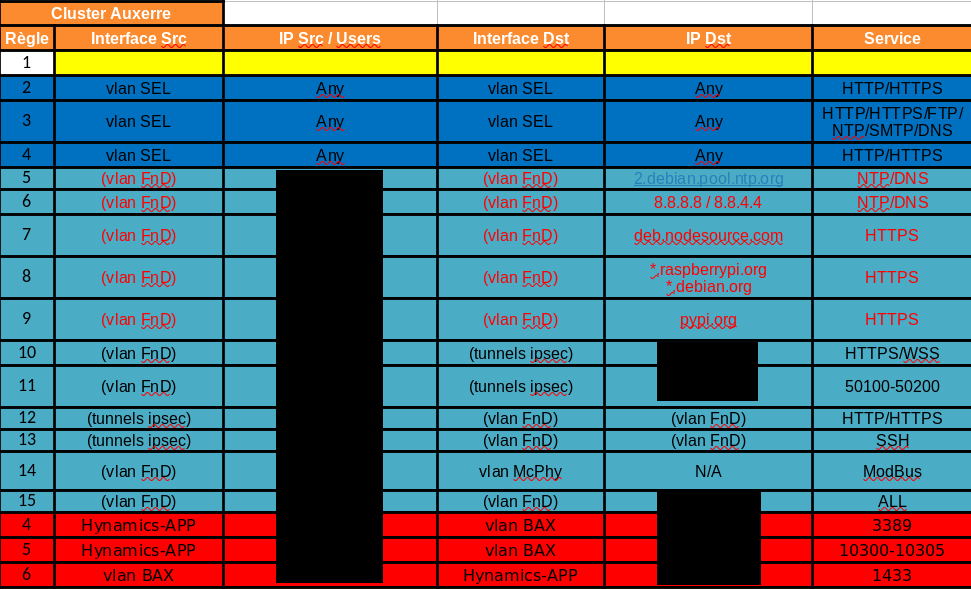
\includegraphics[width = \linewidth]{img/doc-hy/collect.png}
    \caption{Extrait de la Matrice de flux du fichier de collecte}%
    \label{fig:doc-hy/collect}
\end{figure}

\begin{figure}[h!]
    \centering
    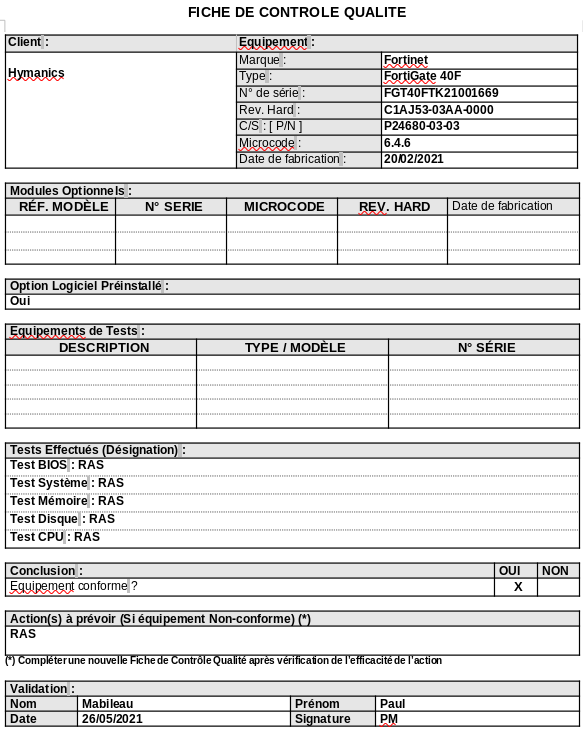
\includegraphics[width = \linewidth]{img/doc-hy/fcq.png}
    \caption{Exemple de Fiche Contrôle Qualité}%
    \label{fig:doc-hy/fcq}
\end{figure}

\begin{figure}[h!]
    \centering
    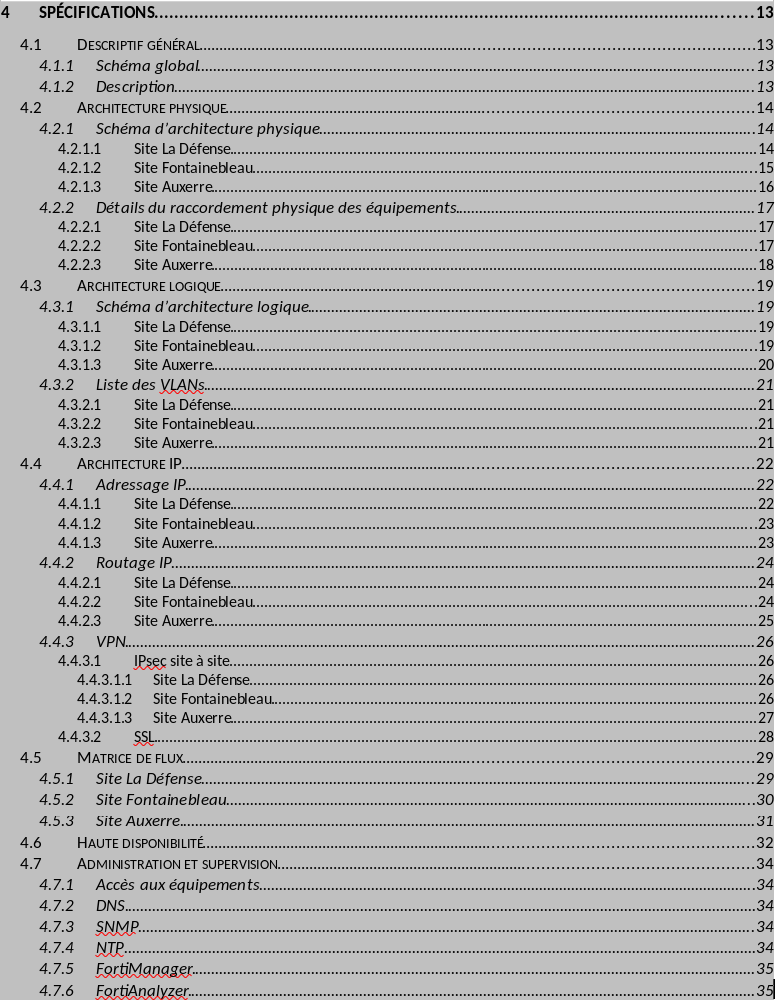
\includegraphics[width = \linewidth]{img/doc-hy/dsd.png}
    \caption{Extrait du plan pour le \gls{dsd} du projet Hynamics}%
    \label{fig:doc-hy/dsd}
\end{figure}

\begin{figure}[h!]
    \centering
    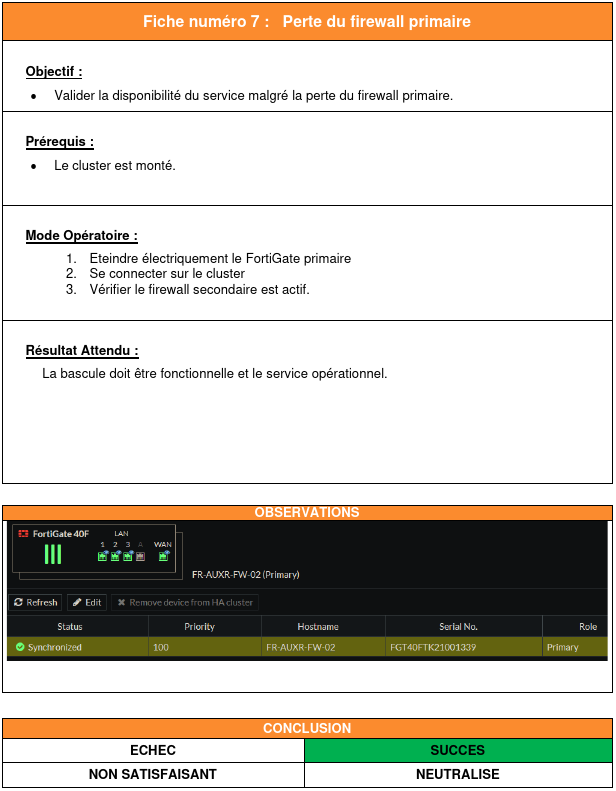
\includegraphics[width = \linewidth]{img/doc-hy/dtv.png}
    \caption{Exemple de fiche de test du \gls{dtv} d'Auxerre}%
    \label{fig:doc-hy/dtv}
\end{figure}

\begin{figure}[h!]
    \centering
    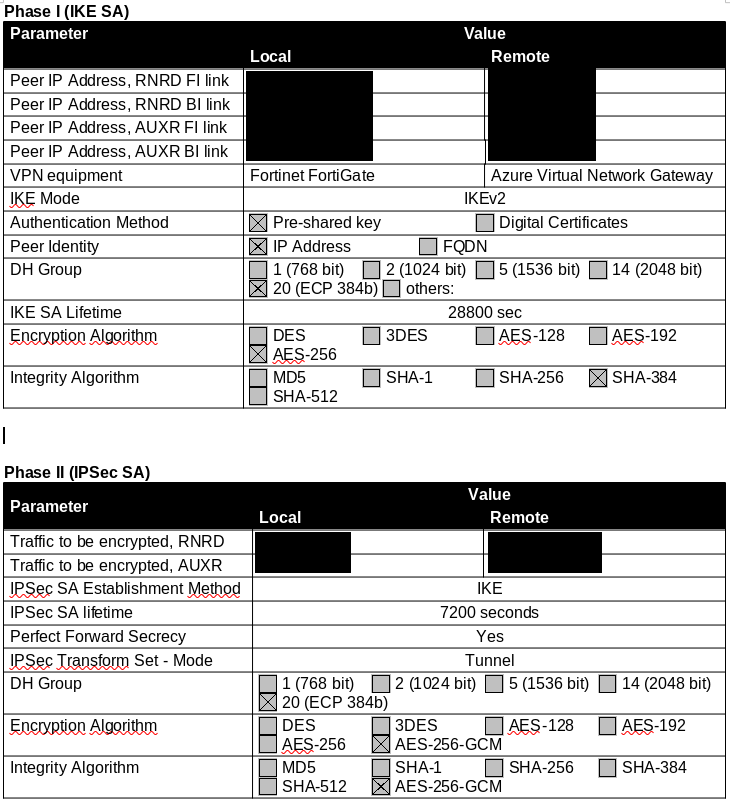
\includegraphics[width = \linewidth]{img/doc-hy/ipsec-tun.png}
    \caption{Exemple de fiche tunnel communiquée au partenaire BaxEnergy}%
    \label{fig:doc-hy/ipsec-tun}
\end{figure}

\section{\acrlong{fgt}}%
\label{sec:annexes::fgt}

\begin{figure}[h!]
    \centering
    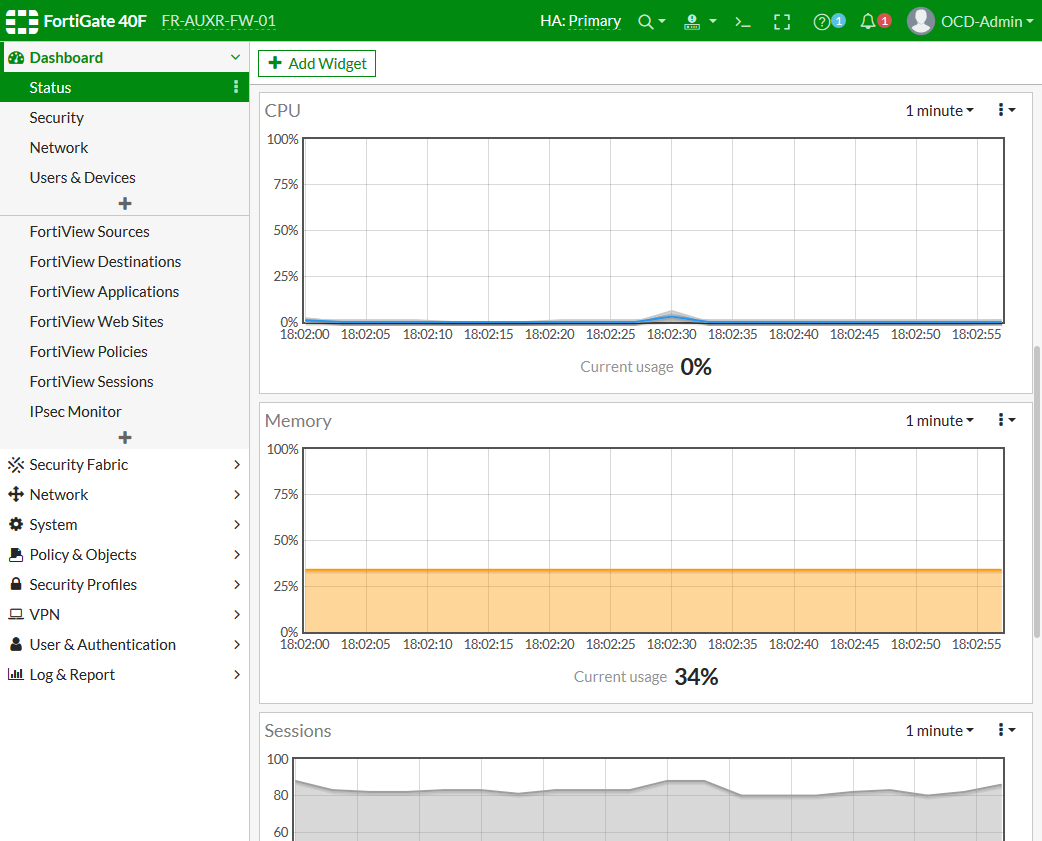
\includegraphics[width = \linewidth]{img/fgt-auxr/dashboard.png}
    \caption{Tableau de bord de l'interface Web d'un \acrlong{fgt}}%
    \label{fig:fgt-auxr/dashboard.png}
\end{figure}

\section{\acrlong{fmg}}%
\label{sec:annexes::fmg}

\begin{figure}[h!]
    \centering
    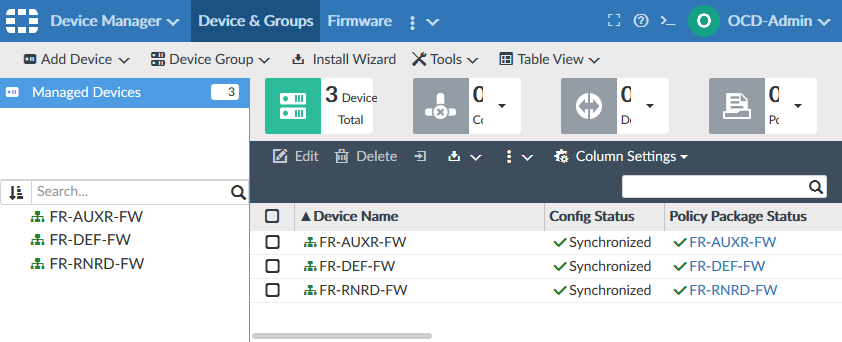
\includegraphics[width = \linewidth]{img/fmg/device-manager.png}
    \caption{Vue du gestionnaire des appareils configurés par un \acrlong{fmg}}%
    \label{fig:fmg/device-manager.png}
\end{figure}

\begin{figure}[h!]
    \centering
    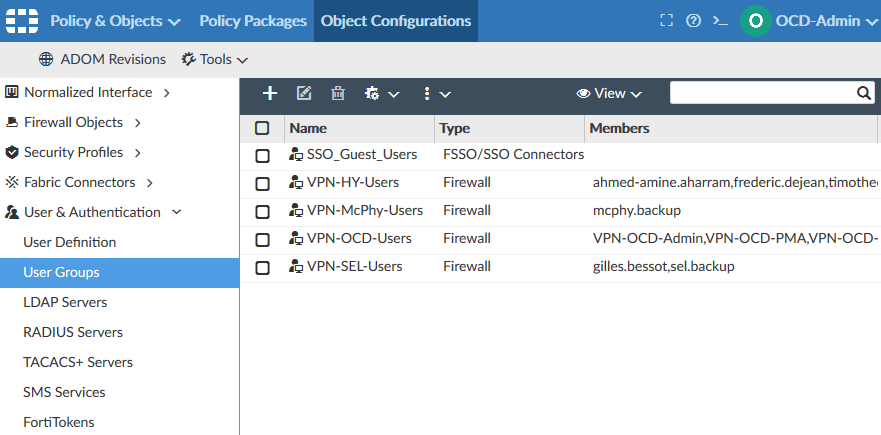
\includegraphics[width = \linewidth]{img/fmg/user-groups.png}
    \caption{Vue des groupes d'utilisateurs sous \acrlong{fmg}}%
    \label{fig:fmg/user-groups}
\end{figure}

\begin{figure}[h!]
    \centering
    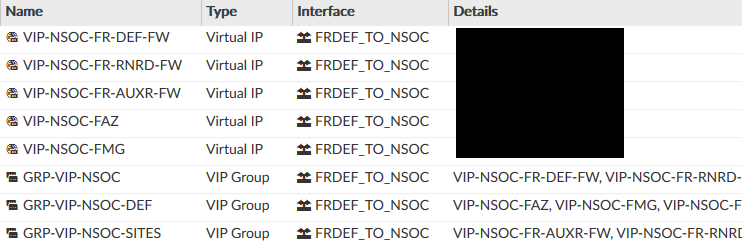
\includegraphics[width = \linewidth]{img/fmg/vips.png}
    \caption{Liste des VIPs configurées par et pour le \gls{run}}%
    \label{fig:fmg/vips.png}
\end{figure}

Comme le montre la Figure~\ref{fig:fmg/vips.png}, des VIPs ont été configurées
sur les pares-feux. Une \textit{Virtual IP address} ou <<adresse IP virtuelle>>
est une fonctionnalité proposées par de nombreux équipements réseau et qui
permet de faire écouter le système d'exploitation sur une certaine interface
mais avec une adresse potentiellement autre que celle de l'interface. Une
configuration possible est de rediriger tout paquet y arrivant avec l'adresse
VIP configurée comme adresse destination vers une autre adresse dans le réseau.
Il est aussi possible de faire ceci en fonction du contenu, ce qui peut être
utilisé pour mettre en place des formes de passerelles de redirection. La
première option a été choisie par le \gls{run} car les adresses des interfaces
\gls{vlan} dans les sous-réseaux dédiés au client, à l'administration et à la
supervision rentraient en conflit avec le plan d'adressage interne au \gls{soc}
et à \gls{ocd}. Ces VIPs leur ont donc permis de joindre les machines en
question mais comme si elles étaient directement dans les sous-réseaux qu'ils
avaient choisis au lieu de celui effectivement utilisé.

\section{Résumé des finances}%
\label{sec:annexes::finances-ocd}

\begin{longtable}{|l|r|r|r|r|}
    \hline{}
    \textbf{Performance} & \textbf{2020} & \textbf{2019} & \textbf{2018} &
    \textbf{2017} \\ \hline{}
        Chiffre d'affaires (\texteuro) & 301M & 274M & 219M & 191M \\ \hline{}
        Marge brute (\texteuro) & 204M & 179M & 153M & 126M \\ \hline{}
        EBITDA --- EBE (\texteuro) & 12,5M & 13,3M & 8,97M & 5,94M \\ \hline{}
        Résultat d'exploitation (\texteuro)
            & 3,63M & 4,8M & 1,43M & 1,2M \\ \hline{}
        Résultat net (\texteuro) & 1,83M & 2,13M & 883K & 1,39M \\ \hline{}
    \textbf{Croissance} & \textbf{2020} & \textbf{2019} & \textbf{2018} &
    \textbf{2017} \\ \hline{}
        Taux de croissance du CA (\%) & 9,8 & 25,1 & 14,8 & 35,6 \\ \hline{}
        Taux de marge brute (\%) & 67,7 & 65,2 & 69,7 & 65,8 \\ \hline{}
        Taux de marge d'EBITDA (\%) & 4,2 & 4,8 & 4,1 & 3,1 \\ \hline{}
        Taux de marge opérationnelle (\%) & 1,2 & 1,8 & 0,7 & 0,6 \\ \hline{}
    \textbf{Gestion BFR} & \textbf{2020} & \textbf{2019} & \textbf{2018} &
    \textbf{2017} \\ \hline{}
        BFR (\texteuro) & 38,4M & 40,8M & 2,07M & 7,33M \\ \hline{}
        BFR exploitation (\texteuro) & 55,8M & 69,9M & 55,6M & 58,2M \\ \hline{}
        BFR hors exploitation (\texteuro) & -17,4M
            & -29,1M & -53,5M & -50,9M \\ \hline{}
        BFR (j de CA) & 46,6 & 54,3 & 3,4 & 14 \\ \hline{}
        BFR exploitation (j de CA) & 67,7 & 93,1 & 92,6 & 111 \\ \hline{}
        BFR hors exploitation (j de CA) & -21,1
            & -38,8 & -89,2 & -97,4 \\ \hline{}
        Délai de paiement clients (j) & 168 & 194 & 176 & 199 \\ \hline{}
        Délai de paiement fournisseurs (j) & 173 & 175 & 140 & 142 \\ \hline{}
        Ratio des stocks / CA (j) & 12,9 & 16,7 & 10,9 & 7,7 \\ \hline{}
    \textbf{Autonomie financière} & \textbf{2020} & \textbf{2019} &
    \textbf{2018} & \textbf{2017} \\ \hline{}
        Capacité d'autofinancement (\texteuro)
            & 10,8M & 10,6M & 8,27M & 5,28M \\ \hline{}
        Capacité d'autofinancement / CA (\%) & 3,6 & 3,9 & 3,8 & 2,8 \\ \hline{}
        Fonds de roulement net global (\texteuro)
            & 41,2M & 43M & 6,02M & 10,9M \\ \hline{}
        Couverture du BFR & 1,1 & 1,1 & 2,9 & 1,5 \\ \hline{}
        Trésorerie (\texteuro) & 2,96M & 2,31M & 3,98M & 3,48M \\ \hline{}
        Dettes financières (\texteuro) & 40M & 50,8M & 16M & 21M \\ \hline{}
        Capacité de remboursement & 3,4 & 4,6 & 1,5 & 3,3 \\ \hline{}
        Ratio d'endettement (Gearing) & 0,5 & 0,7 & 0,2 & 0,3 \\ \hline{}
        Autonomie financière (\%) & 22,9 & 22,8 & 29,5 & 30,2 \\ \hline{}
        Taux de levier (DFN/EBITDA) & 3 & 3,7 & 1,3 & 3 \\ \hline{}
    \textbf{Solvabilité} & \textbf{2020} & \textbf{2019} & \textbf{2018} &
    \textbf{2017} \\ \hline{}
        État des dettes à 1 an au plus (\texteuro)
            & 199M & 182M & 142M & 131K \\ \hline{}
        Liquidité générale & 1,2 & 1,2 & 1 & 1,04K \\ \hline{}
        Couverture des dettes & 2,3 & 1,9 & 7,1 & 4,6 \\ \hline{}
    \textbf{Rentabilité} & \textbf{2020} & \textbf{2019} & \textbf{2018} &
    \textbf{2017} \\ \hline{}
        Marge nette (\%) & 0,6 & 0,8 & 0,4 & 0,7 \\ \hline{}
        Rentabilité sur fonds propres (\%) & 2,6 & 3,2 & 1,3 & 2,1 \\ \hline{}
        Rentabilité économique (\%) & 0,6 & 0,7 & 0,4 & 0,6 \\ \hline{}
        Valeur ajoutée (\texteuro) & 103M & 94,2M & 77M & 62,6M \\ \hline{}
        Valeur ajoutée / CA (\%) & 34,1 & 34,4 & 35,1 & 32,8 \\ \hline{}
    \textbf{Structure d'activité} & \textbf{2020} & \textbf{2019} &
    \textbf{2018} & \textbf{2017} \\ \hline{}
        Salaires et charges sociales (\texteuro)
            & 89,2M & 78,9M & 66,6M & 55,3M \\ \hline{}
        Salaires / CA (\%) & 29,6 & 28,8 & 30,4 & 29 \\ \hline{}
        Impôts et taxes (\texteuro) & 4,11M & 4,09M & 3,27M & 2,66M \\ \hline
    \caption{Résultats financiers~\cite{finances-ocd}}%
    \label{tab:annexes::finances-ocd::tab}
\end{longtable}


\printbibliography[title = Références]

\listoffigures

\glsaddall{}
\printglossary[type = main]
\printglossary[type = \acronymtype, title = Acronymes]



\end{document}
